%%%%%%%%%%%%%%%%%%%%%%%%%%%%%%%%%%%%%%%%%
% Beamer Presentation
% LaTeX Template
% Version 1.0 (10/11/12)
%
% This template has been downloaded from:
% http://www.LaTeXTemplates.com
%
% License:
% CC BY-NC-SA 3.0 (http://creativecommons.org/licenses/by-nc-sa/3.0/)
%
%%%%%%%%%%%%%%%%%%%%%%%%%%%%%%%%%%%%%%%%%

%----------------------------------------------------------------------------------------
%	PACKAGES AND THEMES
%----------------------------------------------------------------------------------------

\documentclass[10pt]{beamer}

\mode<presentation> {

% The Beamer class comes with a number of default slide themes
% which change the colors and layouts of slides. Below this is a list
% of all the themes, uncomment each in turn to see what they look like.

%\usetheme{default}
%\usetheme{AnnArbor}
%\usetheme{Antibes}
%\usetheme{Bergen}
%\usetheme{Berkeley}
%\usetheme{Berlin}
%\usetheme{Boadilla}
%\usetheme{CambridgeUS}
%\usetheme{Copenhagen}
%\usetheme{Darmstadt}
%\usetheme{Dresden}
%\usetheme{Frankfurt}
%\usetheme{Goettingen}
%\usetheme{Hannover}
%\usetheme{Ilmenau}
%\usetheme{JuanLesPins}
%\usetheme{Luebeck}
%\usetheme{Madrid}
\usetheme{Malmoe}
%\usetheme{Marburg}
%\usetheme{Montpellier}
%\usetheme{PaloAlto}
%\usetheme{Pittsburgh}
%\usetheme{Rochester}
%\usetheme{Singapore}
%\usetheme{Szeged}
%\usetheme{Warsaw}

% As well as themes, the Beamer class has a number of color themes
% for any slide theme. Uncomment each of these in turn to see how it
% changes the colors of your current slide theme.

\colorlet{beamer@blendedblue}{blue!40!black}
%\usecolortheme{albatross}
%\usecolortheme{beaver}
%\usecolortheme{beetle}
%\usecolortheme{crane}
%\usecolortheme{dolphin}
%\usecolortheme{dove}
%\usecolortheme{fly}
%\usecolortheme{lily}
%\usecolortheme{orchid}
%\usecolortheme{rose}
%\usecolortheme{seagull}
%\usecolortheme{seahorse}
%\usecolortheme{whale}
%\usecolortheme{wolverine}

%\setbeamertemplate{footline} % To remove the footer line in all slides uncomment this line
%\setbeamertemplate{footline}[page number] % To replace the footer line in all slides with a simple slide count uncomment this line

%\setbeamertemplate{navigation symbols}{} % To remove the navigation symbols from the bottom of all slides uncomment this line
}

\usepackage{graphicx} % Allows including images
\usepackage{booktabs} % Allows the use of \toprule, \midrule and \bottomrule in tables
\usepackage{algorithm}
\usepackage{algpseudocode}
\usepackage{multirow}
\usepackage{tikz}
\usepackage{xcolor} 
\usetikzlibrary{calc}
\usetikzlibrary{arrows,automata}
\usetikzlibrary{positioning}
\usetikzlibrary{decorations.text}
\usetikzlibrary{decorations.pathmorphing}
\usepackage[english]{babel}
\usepackage[utf8x]{inputenc}
\usepackage{amsmath}
\usepackage[colorinlistoftodos]{todonotes}
\usepackage{algorithm}
\usepackage{algpseudocode}
\usepackage{tikz}
\usetikzlibrary{tikzmark,calc}
\usepackage{mathtools}
\usepackage{amsthm}
\usepackage{subcaption,caption}
\usepackage{bm}
%\usepackage{enumitem}

\usepackage[english]{babel}

% \setlength{\parindent}{2em}
% \setlength{\parskip}{1em}
% \renewcommand{\baselinestretch}{1.6}
\DeclarePairedDelimiter\abs{\lvert}{\rvert}%

% to change colors
\newcommand{\fillcol}{green!10}
\newcommand{\bordercol}{black}
\newcommand\norm[1]{\left\lVert#1\right\rVert}

\newcommand\DrawBox[3][]{%
  \begin{tikzpicture}[remember picture,overlay]
    \draw[overlay,fill=gray!30,#1] 
    ([xshift=-8em,yshift=2.1ex]{pic cs:#2}) 
    rectangle 
    ([xshift=2pt,yshift=-0.7ex]pic cs:#3);
  \end{tikzpicture}%
}

\newcommand*{\captionsource}[2]{%
  \caption[{#1}]{%
    #1%
    \\\hspace{\linewidth}%
    \textbf{Source:} #2%
  }%
}

\DeclareMathOperator*{\argmax}{arg\,max}
\DeclareMathOperator*{\argmin}{arg\,min}
\DeclareMathOperator*{\minimize}{minimize}
\DeclareMathOperator*{\maximize}{maximize}


\algnewcommand\algorithmicinput{\textbf{Input:}}
\algnewcommand\INPUT{\item[\algorithmicinput]}

% \theoremstyle{definition}
% \newtheorem{definition}{Definition}[section]
\theoremstyle{remark}
\newtheorem{remark}{Remark}[section]
%----------------------------------------------------------------------------------------
%	TITLE PAGE
%----------------------------------------------------------------------------------------

\title[Introduction to Reinforcement learning]{Introduction to Reinforcement learning} % The short title appears at the bottom of every slide, the full title is only on the title page

\author{Tri Nguyen} % Your name
\institute[OSU] % Your institution as it will appear on the bottom of every slide, may be shorthand to save space
{
Oregon State University \\ % Your institution for the title page
% \medskip
% \textit{lehoang@oregonstate.edu \endgraf } % Your email address
% }
}
\date{\today} % Date, can be changed to a custom date

\graphicspath{ {images/} }

\makeatletter
\renewcommand{\ALG@beginalgorithmic}{\footnotesize}
\makeatother

\newcounter{saveenumi}
\newcommand{\seti}{\setcounter{saveenumi}{\value{enumi}}}
\newcommand{\conti}{\setcounter{enumi}{\value{saveenumi}}}

\newcommand\numberthis{\addtocounter{equation}{1}\tag{\theequation}} % https://tex.stackexchange.com/questions/42726/align-but-show-one-equation-number-at-the-end 
\setbeamerfont{caption}{size=\scriptsize}
\setbeamertemplate{footline}[frame number]



\begin{document}
\DeclareFontShape{OT1}{cmss}{b}{n}{<->ssub * cmss/bx/n}{}
% \newtheorem{theorem}{Theorem}[section]
% \newtheorem{corollary}{Corollary}[theorem]
% \newtheorem{lemma}[theorem]{Lemma}
%------------------------------------------------
\begin{frame}
\titlepage % Print the title page as the first slide
\end{frame}
%------------------------------------------------
%------------------------------------------------

%------------------------------------------------
%\begin{frame}
%\frametitle{Contents} % Table of contents slide, comment this block out to remove it
%\tableofcontents % Throughout your presentation, if you choose to use \section{} and \subsection{} commands, these will automatically be printed on this slide as an overview of your presentation
%\end{frame}
%------------------------------------------------
%------------------------------------------------

%----------------------------------------------------------------------------------------
%	PRESENTATION SLIDES
%----------------------------------------------------------------------------------------

%\section{Description}
% \begin{frame}
% \frametitle{Goals}
% \begin{itemize}
%     \item The essential difference of RL compared to other learning regime
%     \item Concise mathematical framework for problem settings, include notation and graphical representation
%     \item Of course, some examples 
%     \item Let see how many slides to cover these contents
% \end{itemize}
% \end{frame}

\begin{frame}
    \frametitle{Reinforcement Learning (RL)}
    \begin{table}[c]
        \begin{tabular}{c|p{3cm}|p{4cm}}
            & With teacher & Without teacher \\
            \hline
            Passive & Supervised & Self-(un)supervised \\
                    & Learning & Learning \\
            \hline
            Active & \textbf{Reinforcement} & Intrinsic Motivation \\
                   & \textbf{Learning} & (Exploration) \\ 
            \hline
        \end{tabular}
        \caption{Tutorial - ICML2021}
    \end{table}
    Learning \textbf{what-to-do} from \textbf{interaction} and optimizing \textbf{reward}.
\end{frame}

\begin{frame}
    \setbeamerfont{footnote}{size=\tiny} 
    \frametitle{Problems to cast to RL}
    \begin{figure}[h]
        \begin{subfigure}[t]{0.4\textwidth}
            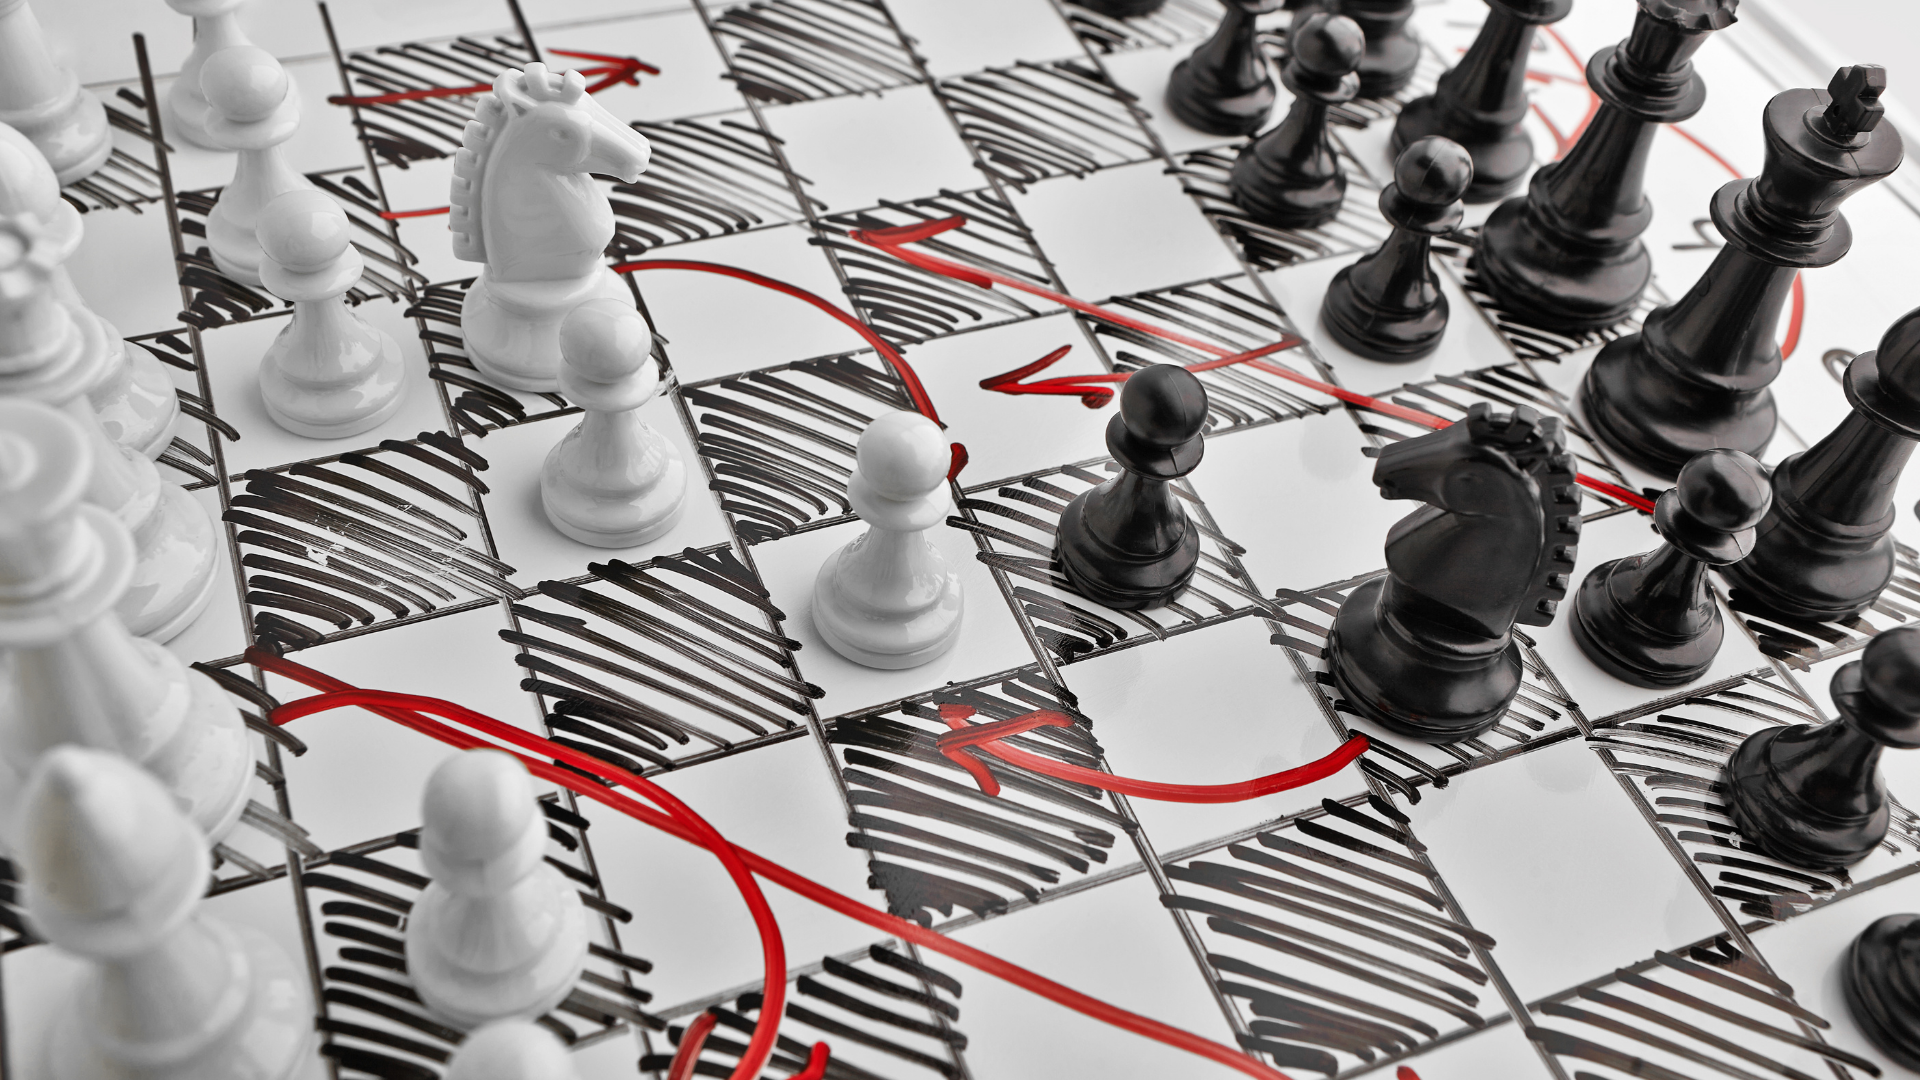
\includegraphics[width=\textwidth]{figures/motivation1.png}
            \caption{Board games}
        \end{subfigure}
        \begin{subfigure}[t]{0.4\textwidth}
            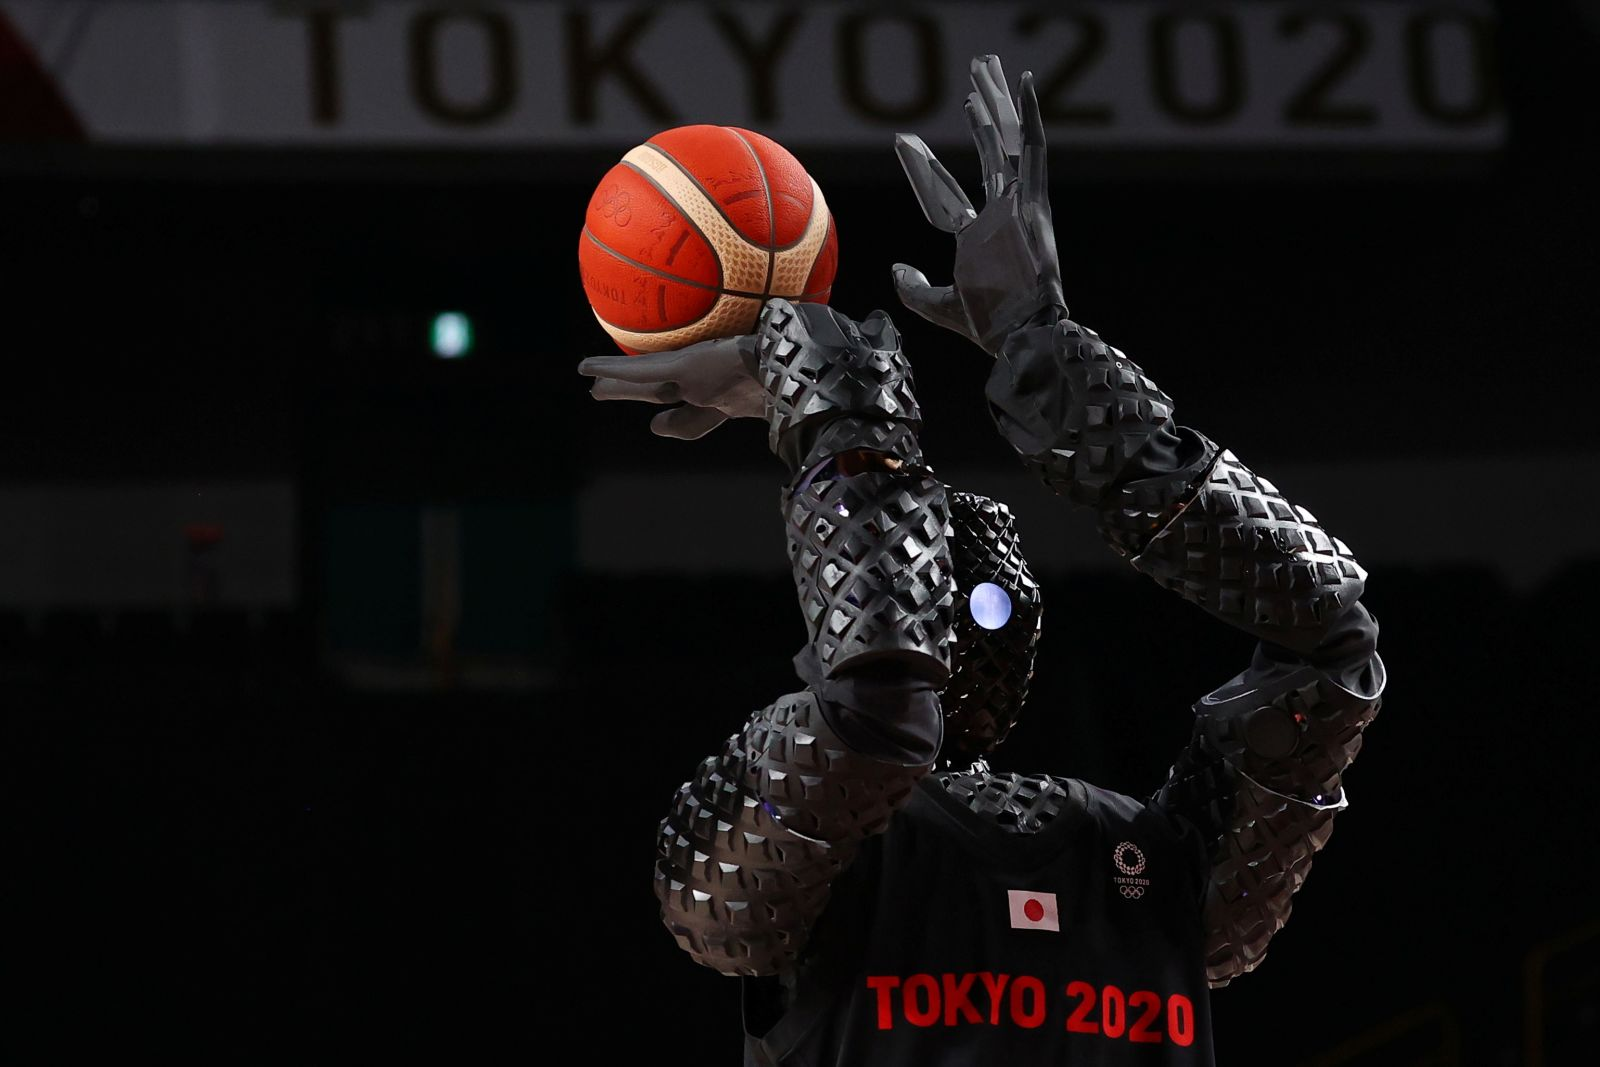
\includegraphics[width=\textwidth]{figures/motivation2.jpg}
            \caption{\href{https://www.youtube.com/watch?v=KH9m0L7F-sE}{Robot manipulation}}
        \end{subfigure}

        \begin{subfigure}[t]{0.4\textwidth}
            
\includegraphics[width=\textwidth]{figures/motivation3.jpg}
            \caption{Real-time strategy games}
        \end{subfigure}
        \begin{subfigure}[t]{0.4\textwidth}
            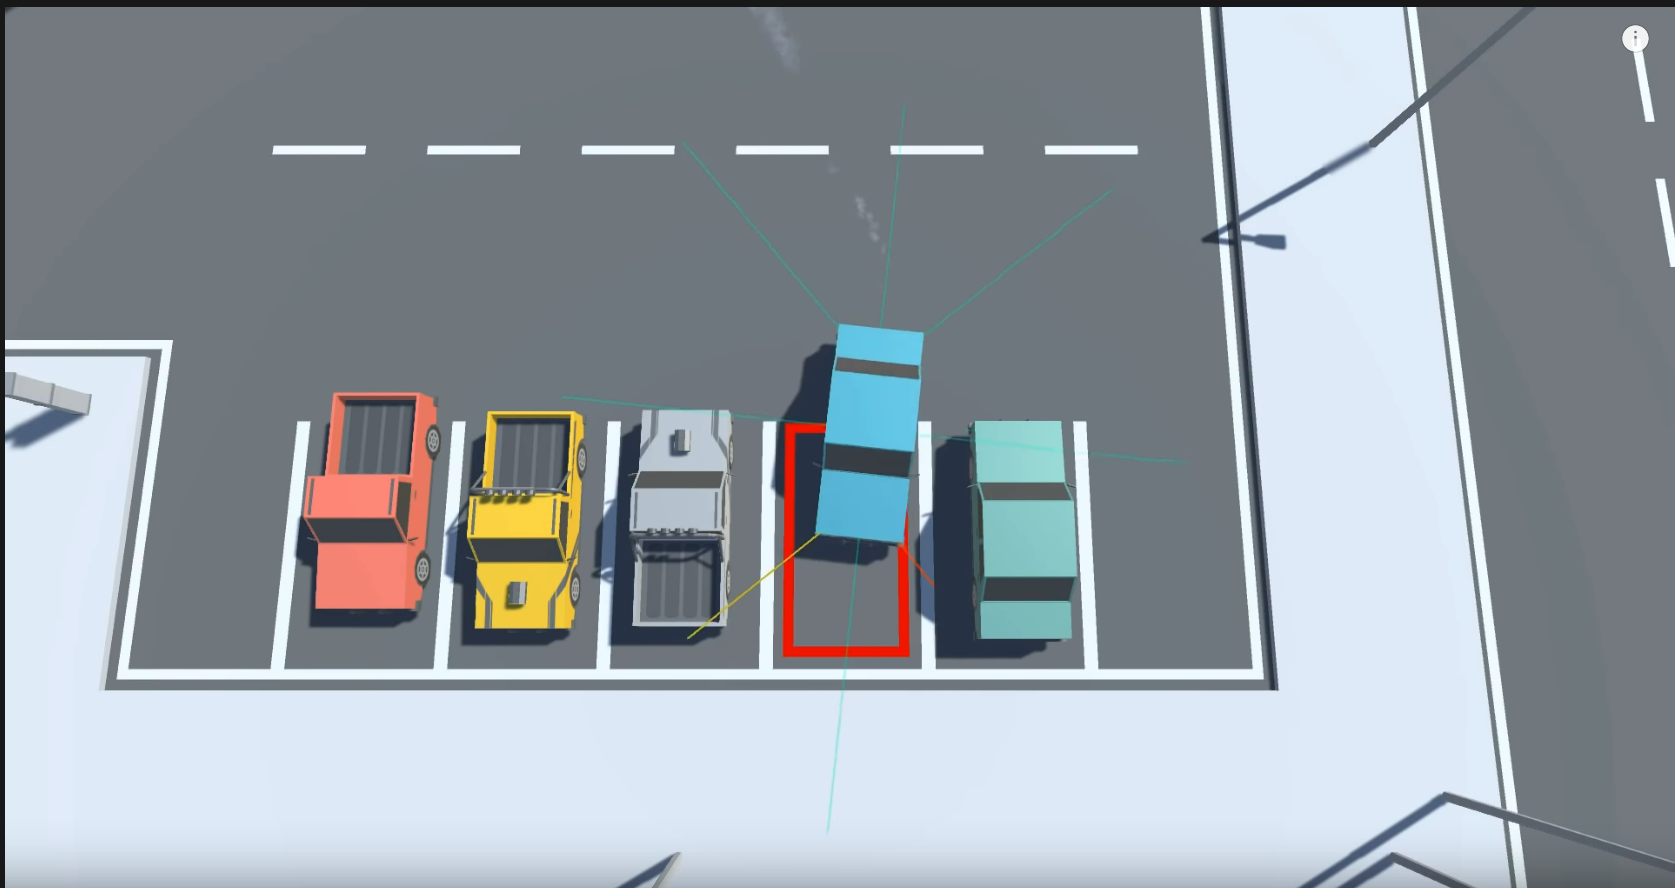
\includegraphics[width=\textwidth]{figures/motivation4.png}
            \caption{\href{https://www.youtube.com/watch?v=VMp6pq6_QjI&t=0s}{Self-driving car}}
        \end{subfigure}
    \end{figure}
    and many more \ldots 
\end{frame}



\begin{frame}
    \begin{figure}
        \begin{subfigure}{0.45\textwidth}
            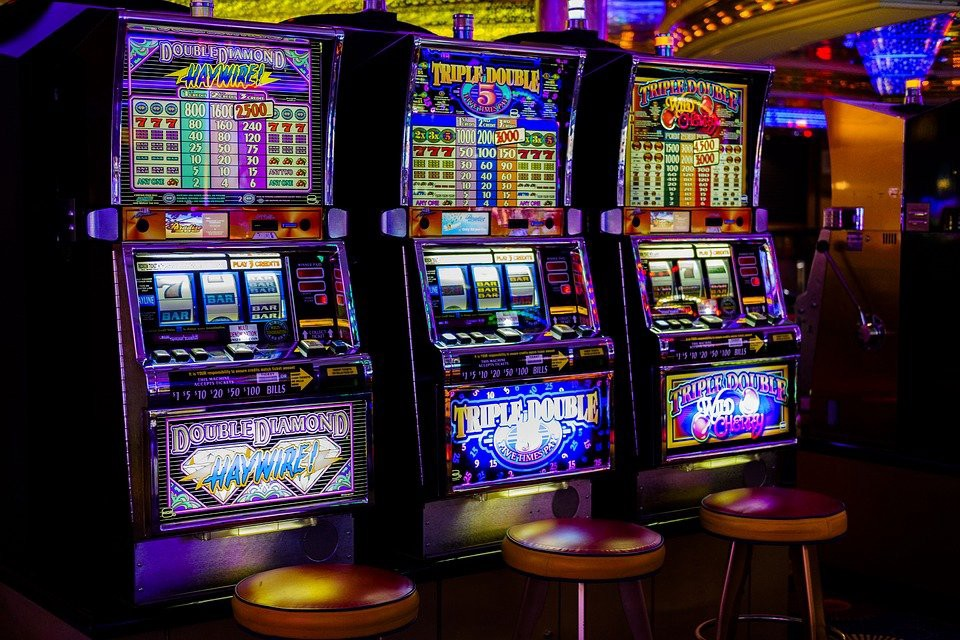
\includegraphics[width=\textwidth]{figures/multiarmed-bandit1.jpg}
        \end{subfigure}
        \begin{subfigure}{0.45\textwidth}
            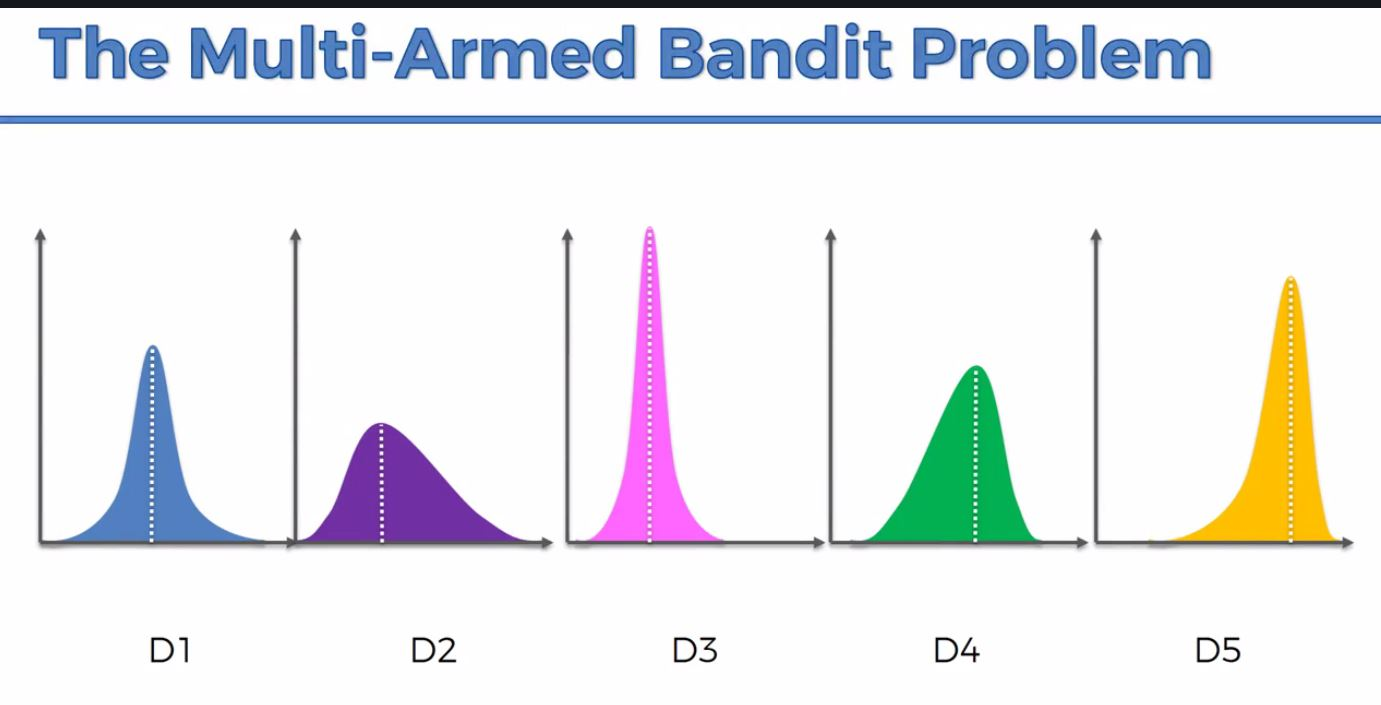
\includegraphics[width=\textwidth]{figures/multiarmed-bandit.jpg}
        \end{subfigure}
    \end{figure}
    Given $n$ bandit machines. You can pull the level of one of them and obsever the result: either nothing or win a fixed amount of cash. Each bandit machine has it owns wining distribution. If you can play M times, what's your strategy to maximize total amount of cash?
    \begin{itemize}
        \item $A_t$ as action picked at step $t$
        \item  $R_t$ as reward received at step  $t$
        \item  Action value: $q_{*}(a) = \mathbb{E}[R_t | A_t = a]$
        \item Estimate action value at step $t$: $Q_t(a)$
    \end{itemize}
    Balancing between exploitation and exploration!
\end{frame}

\begin{frame}
    \frametitle{Baseline: $\epsilon$-greedy Algorithm}
    Estimate $q_{\ast}(a)$ by $Q_n(a) = \dfrac{R_1 + R_2 + \ldots  R_{n-1}}{n-1}$
    \begin{figure}
        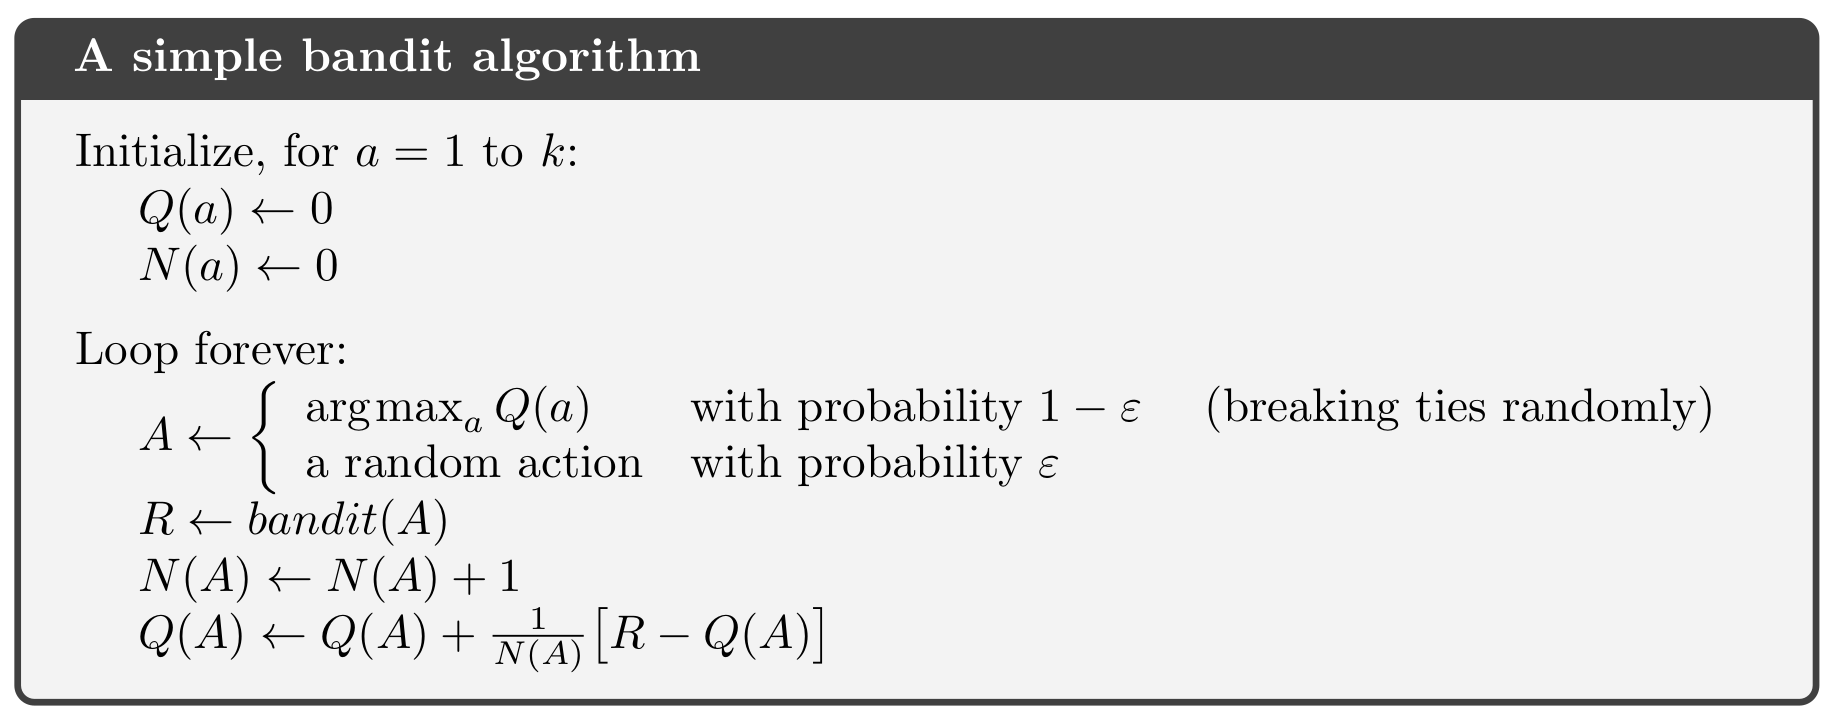
\includegraphics[width=\textwidth]{figures/simple_alg.png}
        \caption{From [Sutton\&Barto]}
    \end{figure}
\end{frame}

\begin{frame}
    \frametitle{Variant 1: Optimistic Initial Values}
    Init $Q(a)$ as a nonzero constant $C > 0$.
    \begin{figure}
        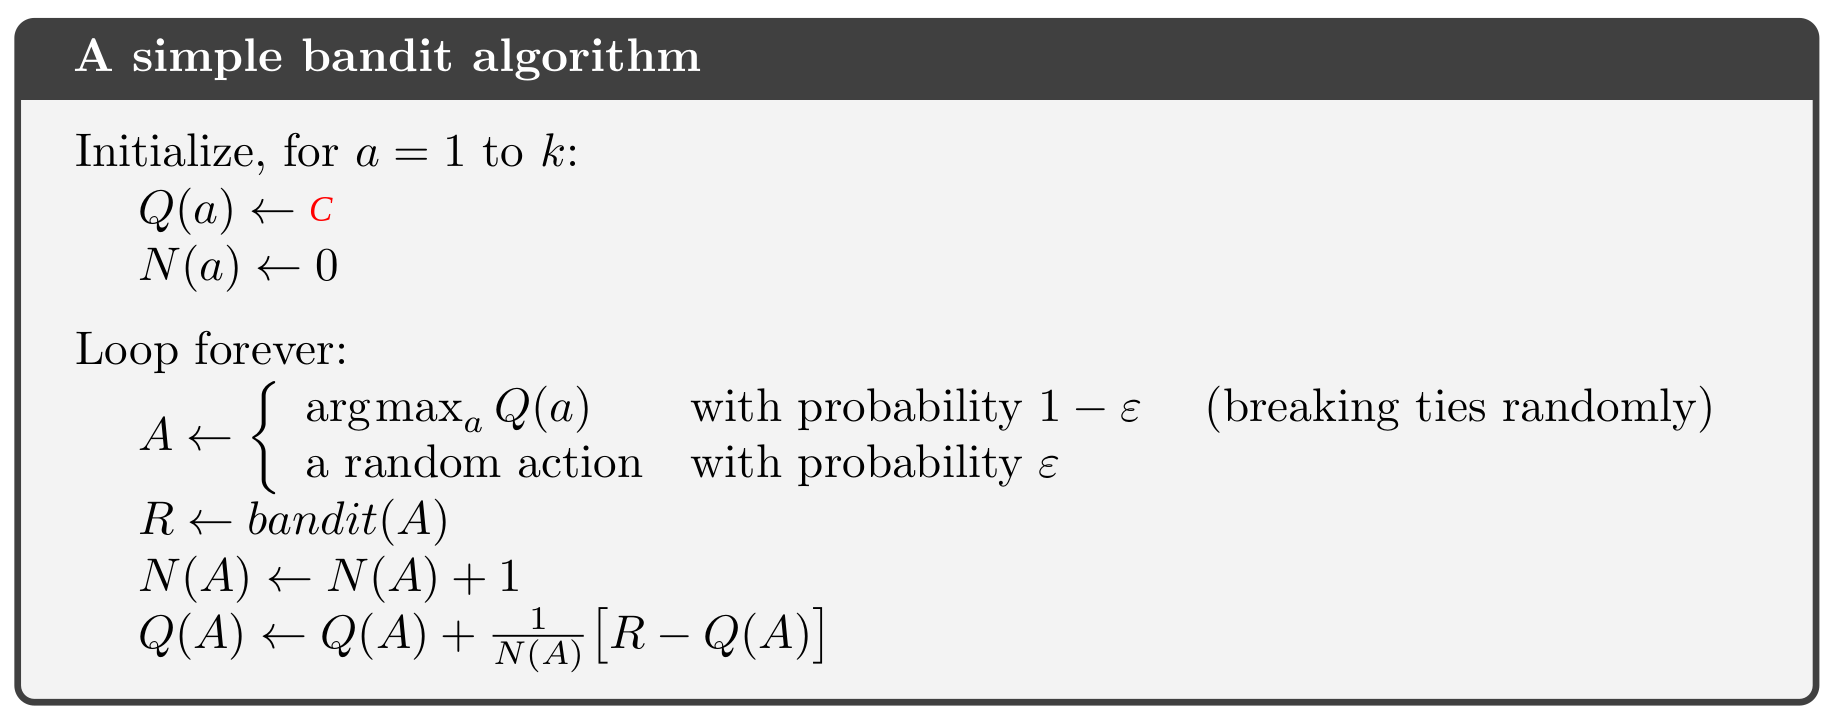
\includegraphics[width=\textwidth]{figures/simple_alg1.png}
        \caption{From [Sutton\&Barto]}
    \end{figure}
\end{frame}

\begin{frame}
    \frametitle{Variant 2: Upper-Confidence-Bound Action Selection (UCB)}
    \begin{figure}
        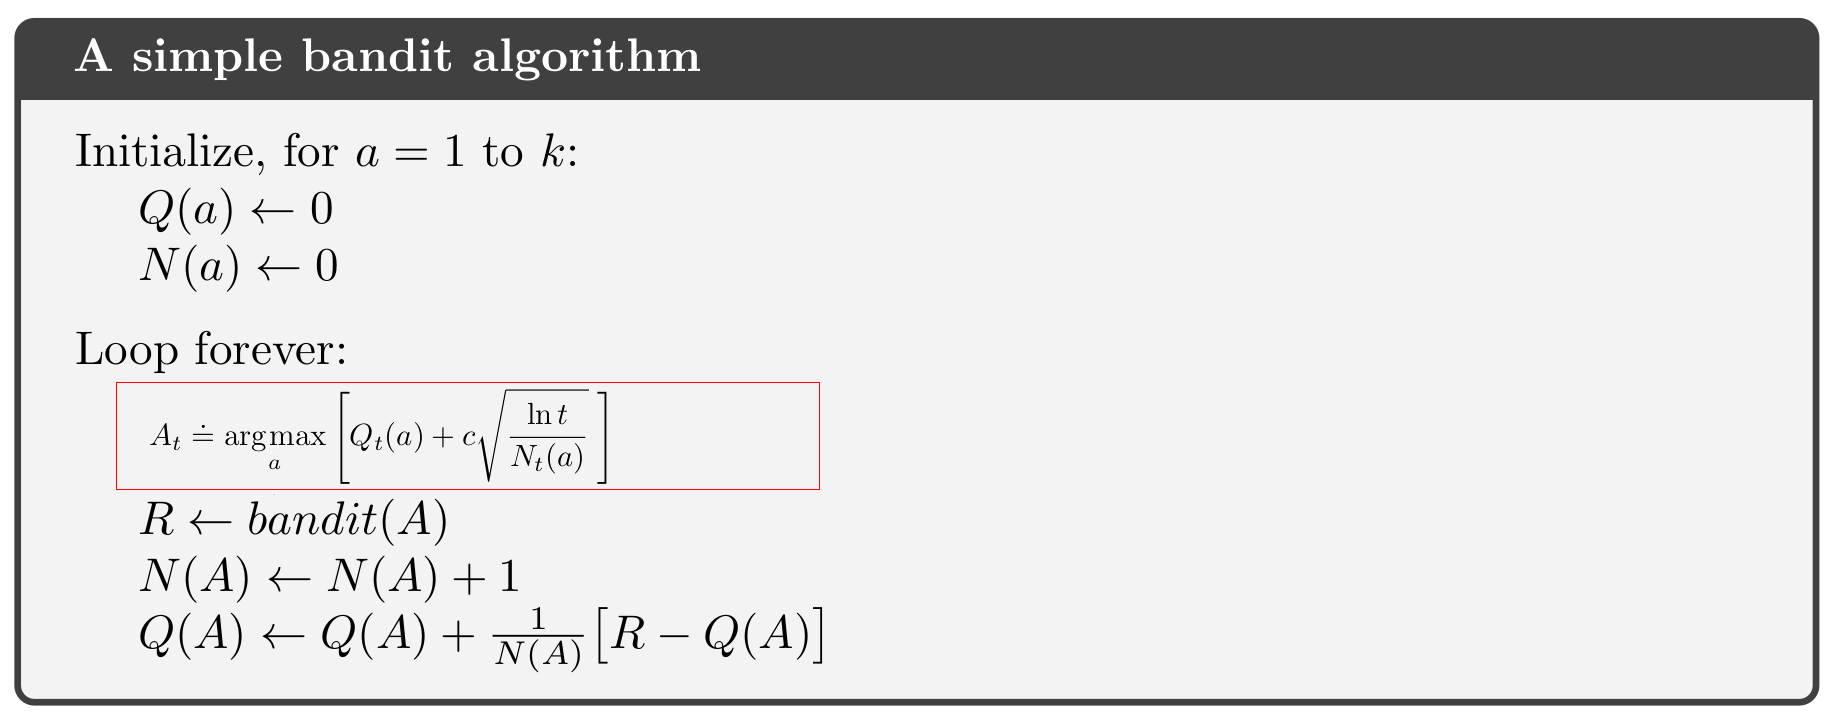
\includegraphics[width=\textwidth]{figures/simple_alg2.png}
        \caption{From [Sutton\&Barto]}
    \end{figure}
\end{frame}

\begin{frame}
    \frametitle{Evaluation}
    \begin{figure}
        \centering
        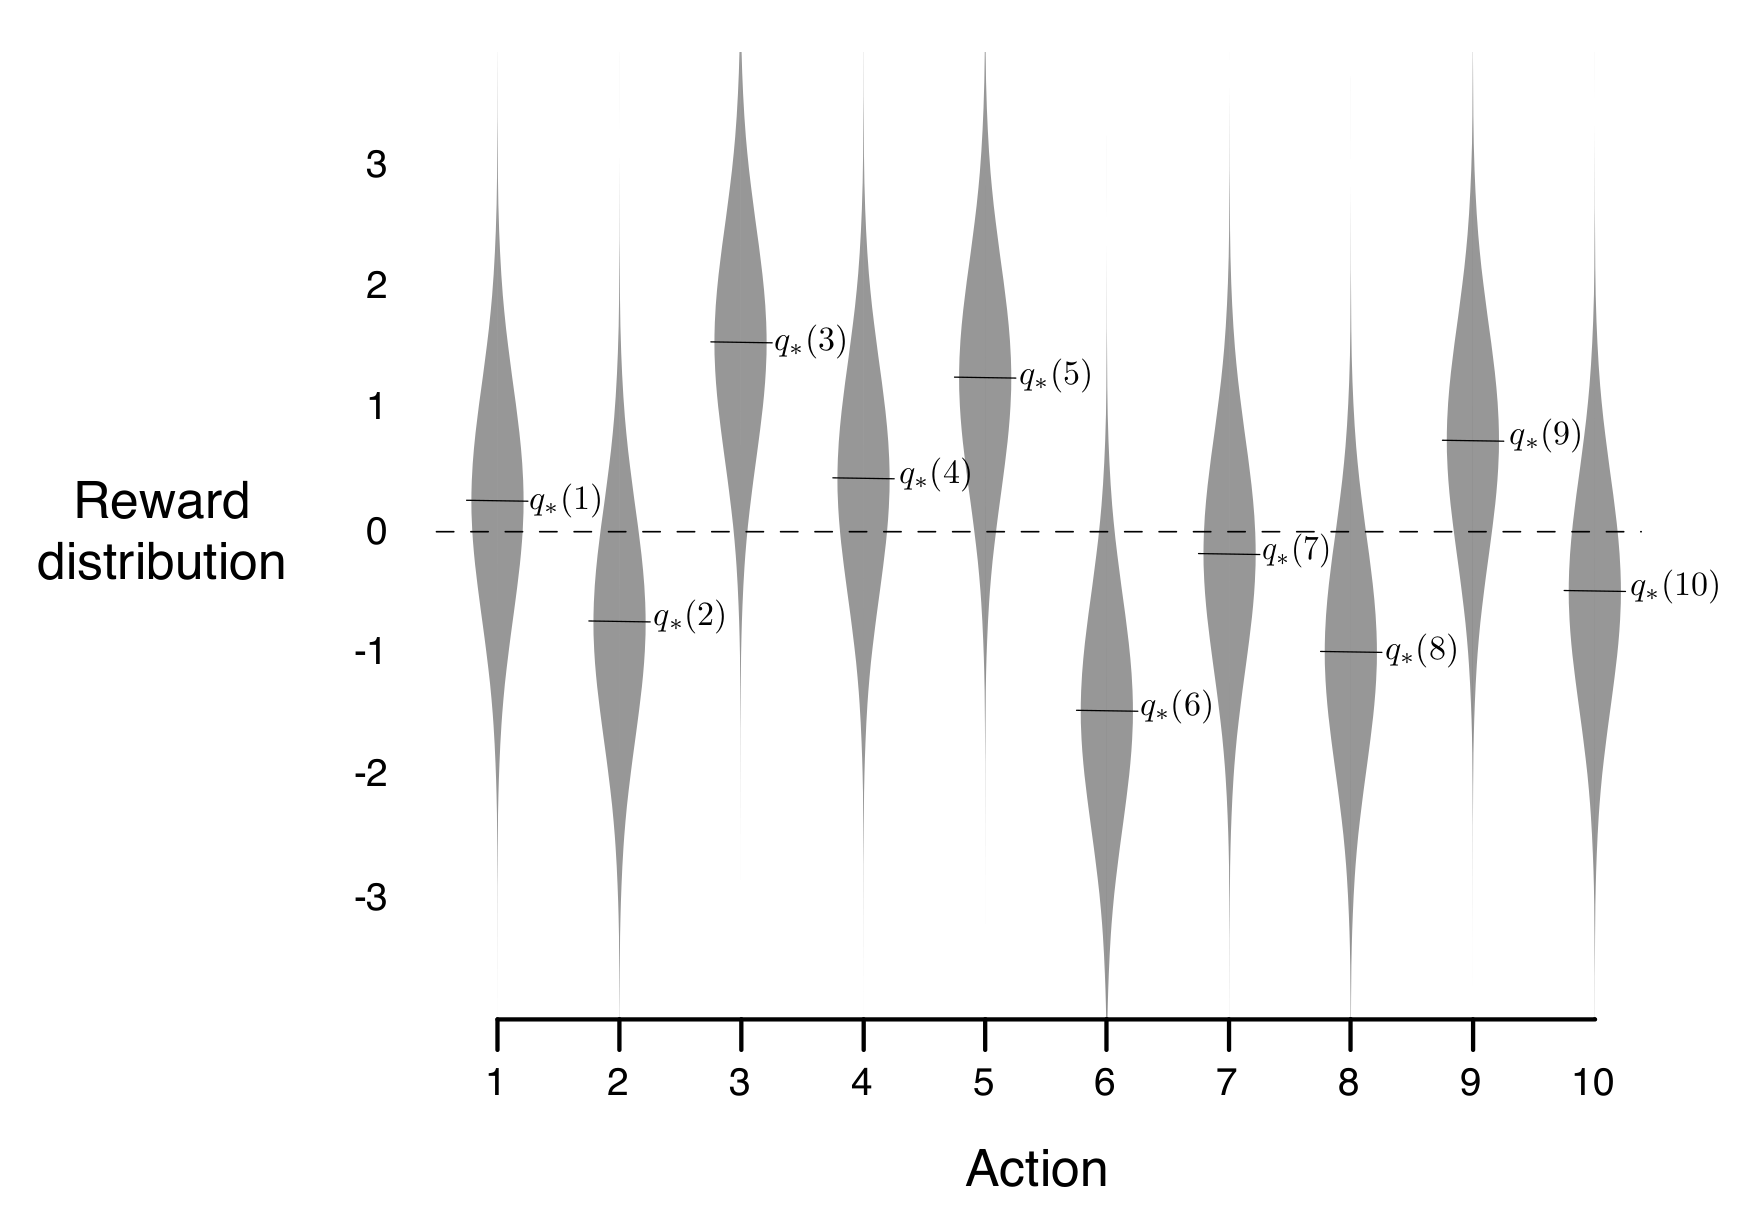
\includegraphics[width=0.6\textwidth]{figures/test_init.png}
        \caption{From [Sutton\&Barto]}
    \end{figure}
    \begin{itemize}
        \item 10-armed bandits
        \item Each $q_{\ast}(a) \sim \mathcal{N}(0, 1)$
        \item And then the actual rewards are drawn from $\mathcal{N}$ with a mean $q_{\ast}(a)$ and unit variance
    \end{itemize}
\end{frame}

\begin{frame}
    The results are averages over 2000 trials.
    \begin{figure}
        \begin{subfigure}{0.45\textwidth}
        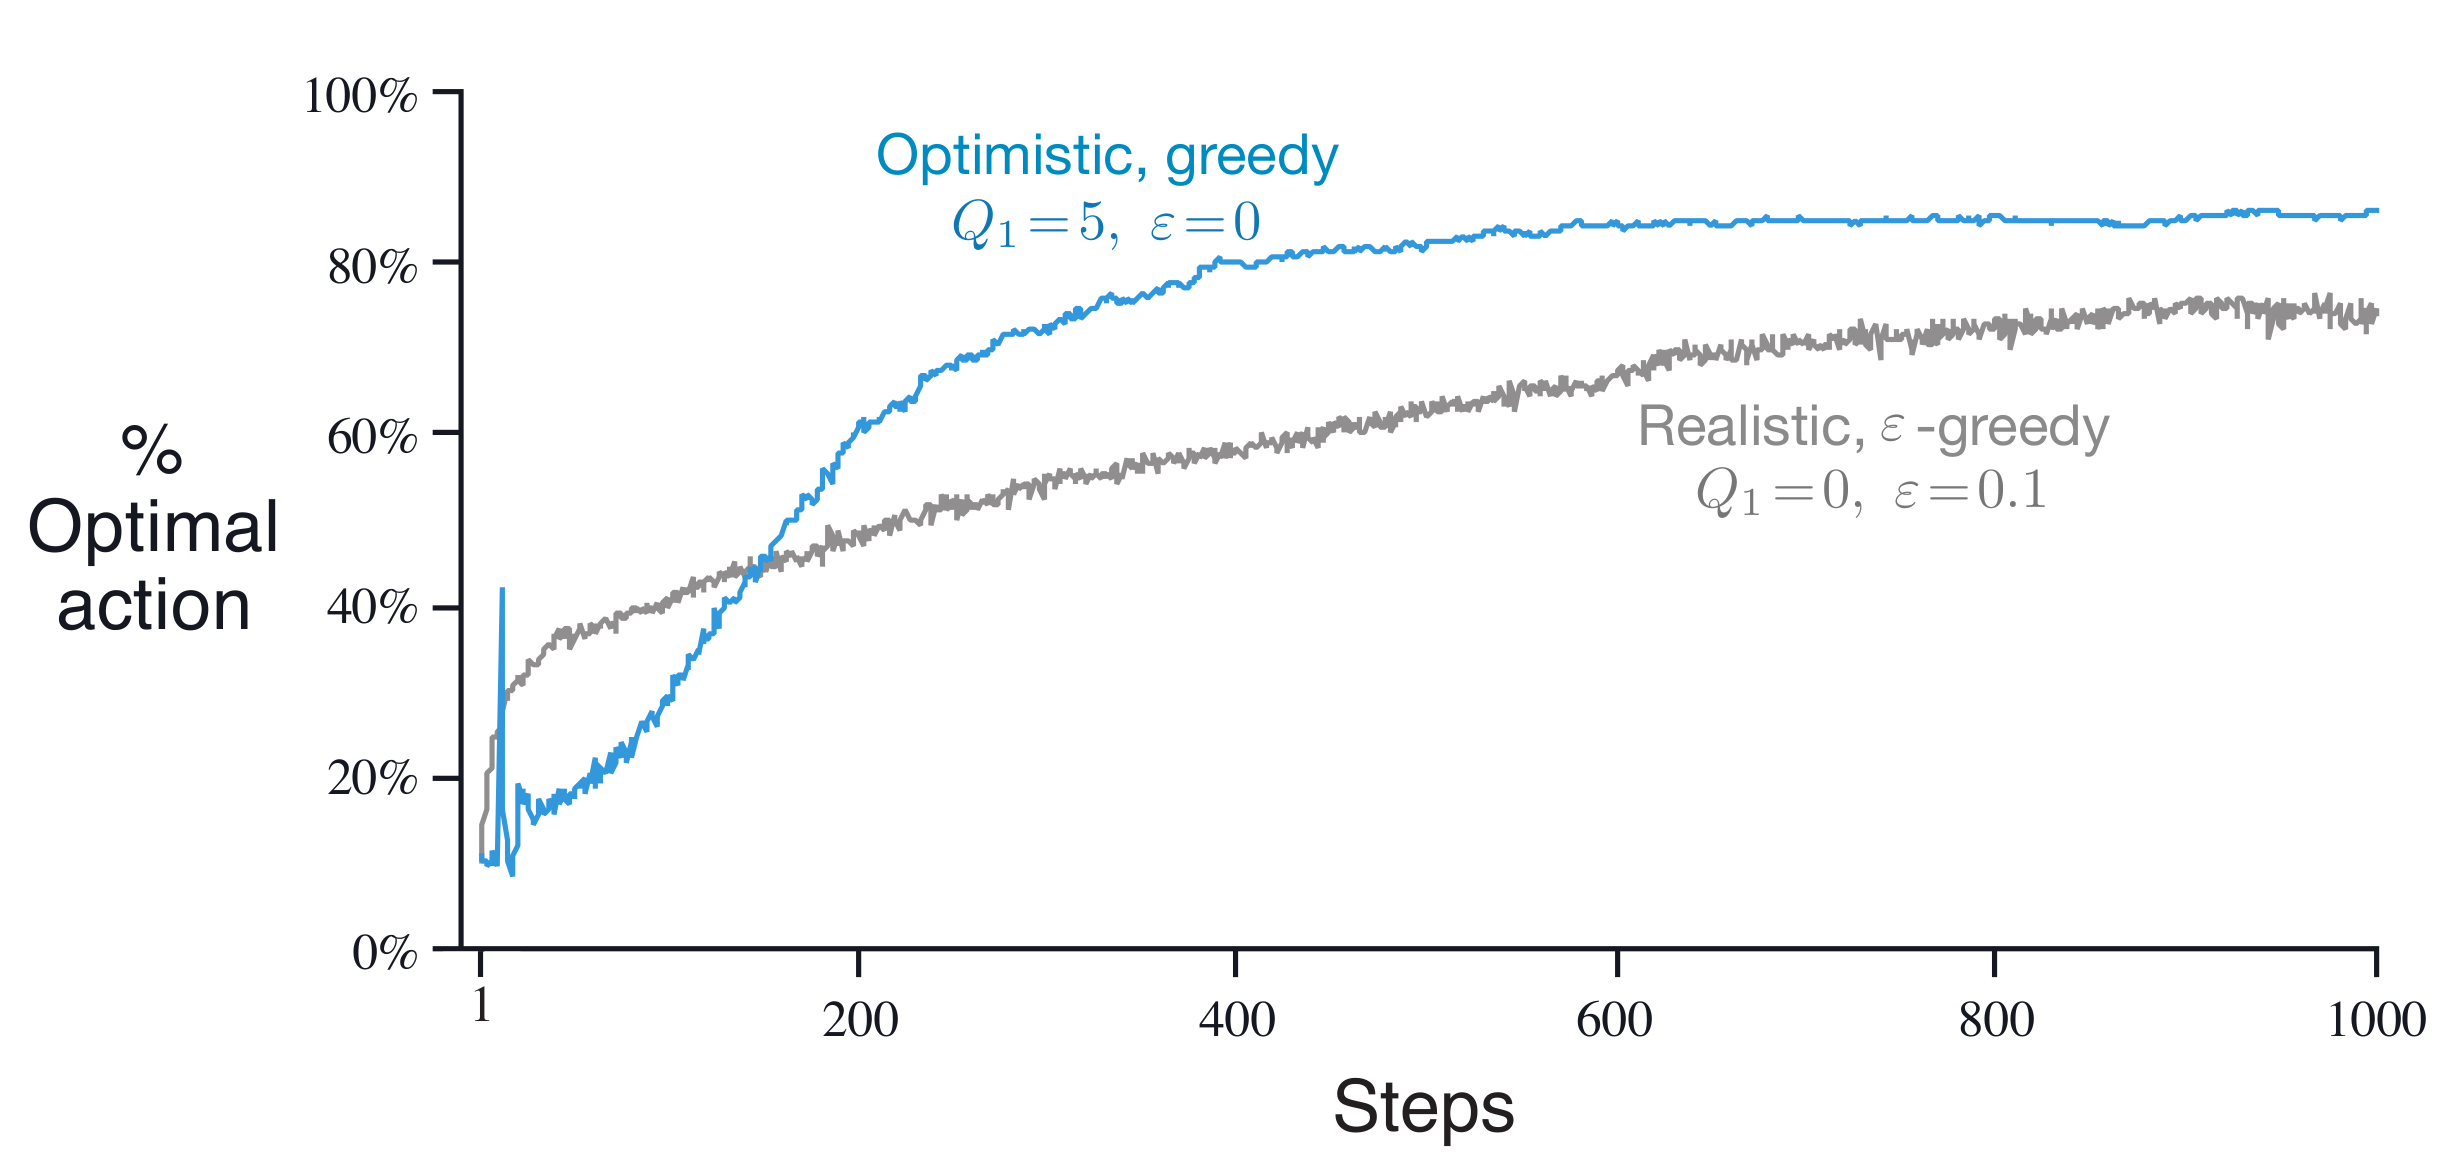
\includegraphics[width=\textwidth]{figures/bandit_vs_1.png}
        \caption{$\epsilon$-greedy v.s Optimistic Initial Value}
        \end{subfigure}
        \begin{subfigure}{0.45\textwidth}
            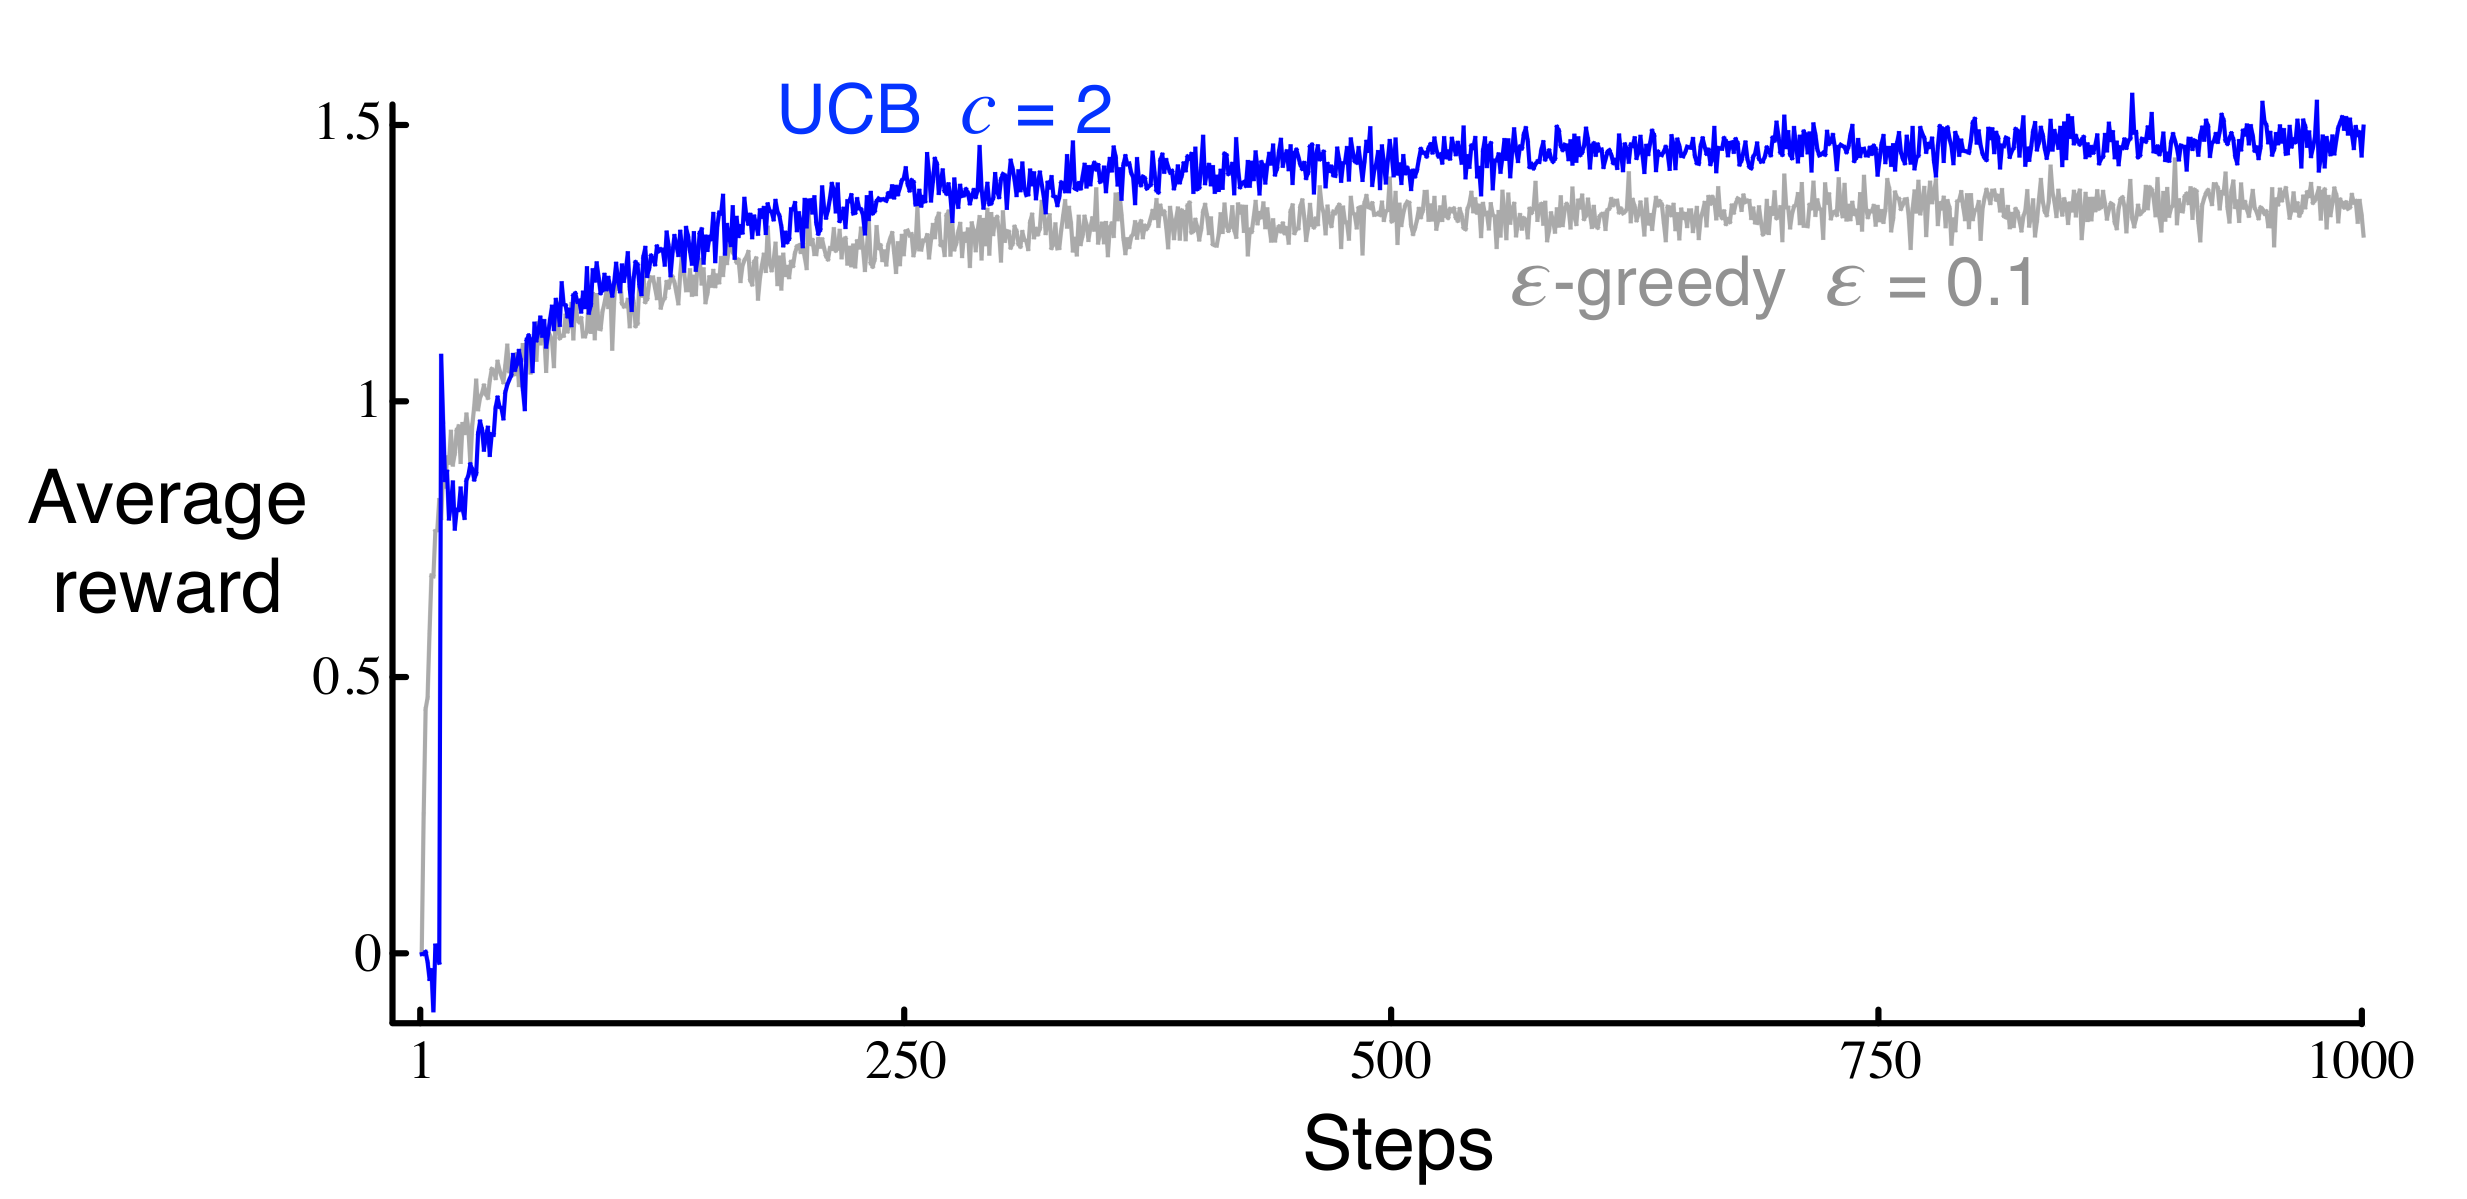
\includegraphics[width=\textwidth]{figures/bandit_vs_2.png}
            \caption{$\epsilon$-greedy v.s UCB}
        \end{subfigure}
    \end{figure}
    Note that in both figures, there is a jump around in early part of the curve.
    \begin{itemize}
        \item In the first $10$ iterations, all actions are seleted once regardless of actual rewards.
        \item After that, $Q_{11}(a)$ might estimate $q_{\ast}(a)$ relatively correct, i.e., $\argmax_a Q_{11}(a) = \argmax_a q_{\ast}(a) $
        \item Then it is likely ($40\%$ ) that an optimal action is picked.
    \end{itemize}
\end{frame}


\begin{frame}
    \frametitle{Reinforcement Learning Framework}
    General question: how to train an agent to archive a goal by interacting with the environment, e.g., train a robot to escape a maze. \\

    RL solves it by using the following framework:
    \begin{figure}
        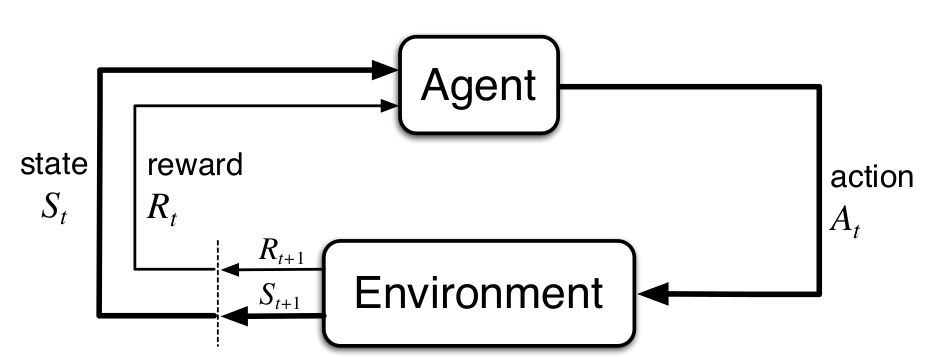
\includegraphics[width=0.4\textwidth]{figures/agent-environment.png}
        \caption{[Sutton\&Barto]}
   \end{figure}
   \textbf{Input of the framework}

   Environment - Agent interation:
   \begin{itemize}
       \item At time step $t$, \textit{agent} at state $S_t$ performs an action $A_t \in \mathcal{A}(S_t)$
       \item The \textit{environment} acts accordingly change to state $S_{t+1}$, emits a reward $R_{t+1}$
       \item \textit{Return}: $G_t = \sum^{\infty}_{k=1} \gamma^{k}R_{t+k+1}$
   \end{itemize}
   \textbf{Output of the framework}

   An agent that acts on the environment so that it maximizes the expectation of \textit{return}, i.e., $ \mathbb{E}[G_t]$.
\end{frame}

\begin{frame}
    \frametitle{Examples of using framework}
    \begin{columns}
    \begin{column}{0.4\textwidth}
        \begin{figure}
            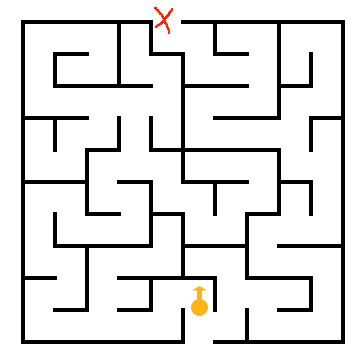
\includegraphics[width=\textwidth]{figures/maze.png}
            \caption{Given a position, find a way to reach the {\color{red} red X}}
        \end{figure}
    \end{column}
    \begin{column}{0.7\textwidth}  %%<--- here
        Goal: Given a position, find a way to reach the {\color{red} red X}

        \begin{itemize}
            \item At time $t$, state $S_t$ is current position
            \item Agent at state $S_t$ can move to any valid directions (direction not break wall)
            \item Environment dynamic: 
                \begin{itemize}
                    \item Agent being at the desired position by 1 unit 
                    \item Emits a reward of $10$ when it reach X, otherwise $0$.
                \end{itemize}
            \item Return $G_t = \sum^{\infty}_{k=1} R_{t+k+1} $.

            Not that we choose $\gamma = 1$, and $T$ is number of time steps until the agent reaches {\color{red} red X}
        \end{itemize}
    \end{column}
    \end{columns}
\end{frame}

\begin{frame}
    \begin{columns}
    \begin{column}{0.4\textwidth}
        \begin{figure}
            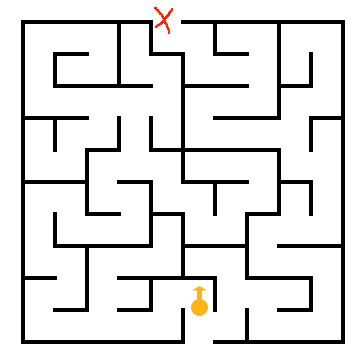
\includegraphics[width=\textwidth]{figures/maze.png}
            \caption{Given a position, find a way to reach the  red X as fast as possible}
        \end{figure}
    \end{column}
    \begin{column}{0.7\textwidth}  %%<--- here
        Goal: Given a position, find a way to reach the red X {\color{red} as fast as possible!}

        \begin{itemize}
            \item At time $t$, state $S_t$ is current position
            \item Agent at state $S_t$ can move to any valid directions (direction not break wall)
            \item Environment dynamic: 
                \begin{itemize}
                    \item Agent being at the desired position by 1 unit 
                    \item Emits a reward of $10$ when it reach X, {\color{red} otherwise $-1$}.
                \end{itemize}
            \item Return $G_t = \sum^{\infty}_{k=1} R_{t+k+1}$.

            Not that we choose $\gamma = 1$, and $T$ is number of time steps until the agent reaches \color{red} red X
        \end{itemize}
    \end{column}
    \end{columns}
\end{frame}


\begin{frame}
    \frametitle{Cart-Pole Problem}
    \begin{columns}
    \begin{column}{0.4\textwidth}
        \begin{figure}
            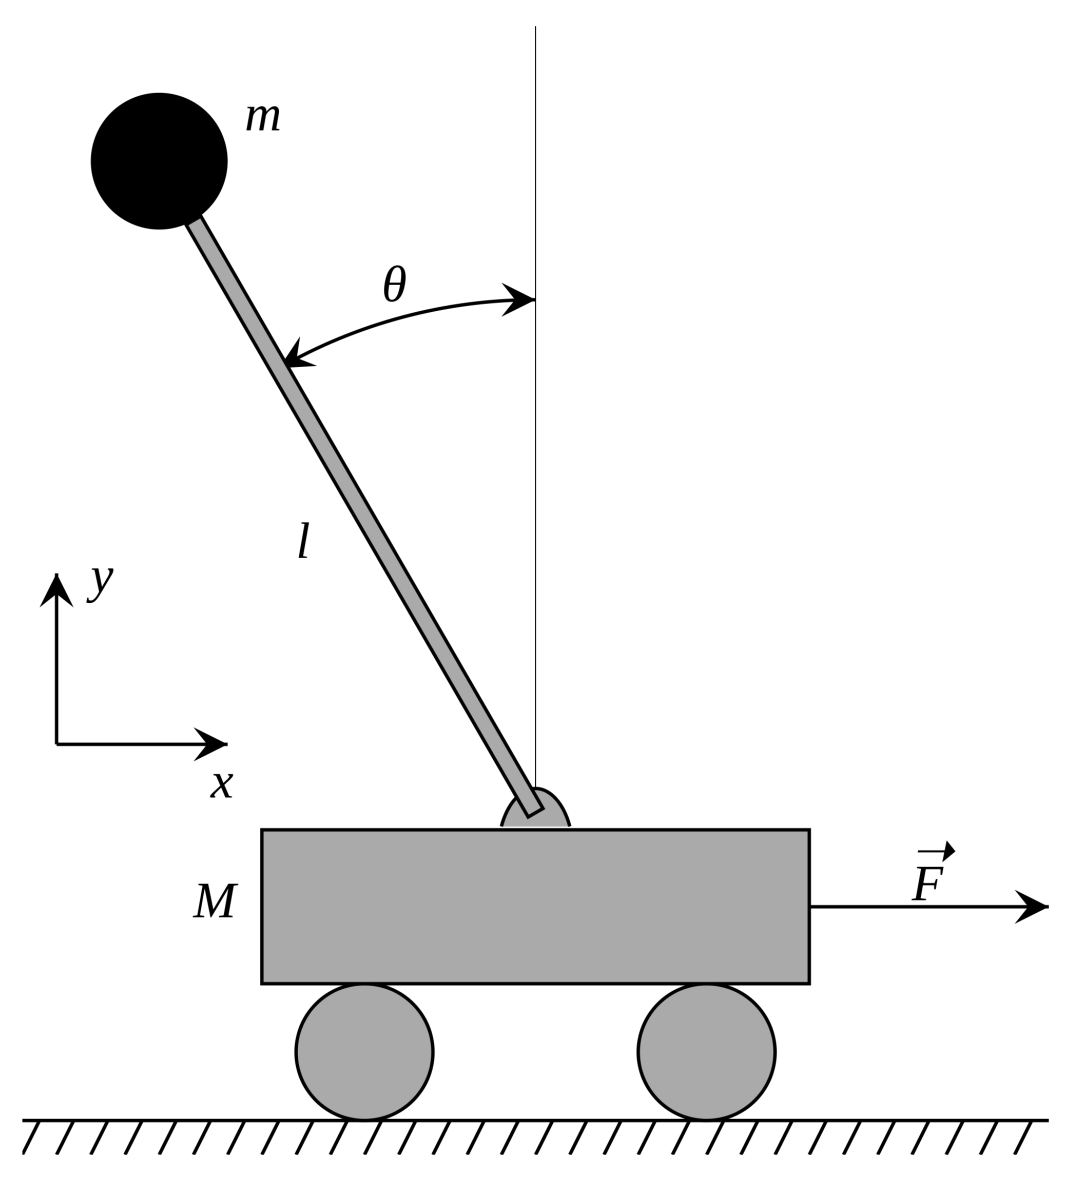
\includegraphics[width=\textwidth]{figures/pole-balance.png}
            \caption{Keep the pole from falling by moving the card horizontally (From Lecture \footnotemark)}
        \end{figure}
    \end{column}
    \begin{column}{0.7\textwidth}  %%<--- here
        Goal: Keep the pole from falling by moving the card horizontally

        \begin{itemize}
            \item At time $t$, state $S_t$ is a collection of \textit{angle, angular speed, position, horizontal vertical}
            \item Agent at state $S_t$ can apply a force horizontally to the cart.
            \item Environment dynamic: 
                \begin{itemize}
                    \item The pole acts accordingly to physical laws.
                    \item Emits a reward of $1$ when the pole is upright, otherwise $-10$.
                    \item Once the pole hits ground, there's no way to make it be upright.
                \end{itemize}
            \item Return $G_t = \sum^{\infty}_{k=1} R_{t+k+1} $.

            Not that we choose $\gamma = 1$, and $T$ is number of time steps until the pole is dropped.
        \end{itemize}
    \end{column}
    \end{columns}

    \footnotetext[1]{Lecture CS231 Stanford - Fei-Fei Li \& Justin Johnson \& Serena Yeung}
\end{frame}

\begin{frame}
    \frametitle{Playing chess}
    \begin{columns}
    \begin{column}{0.4\textwidth}
        \begin{figure}
            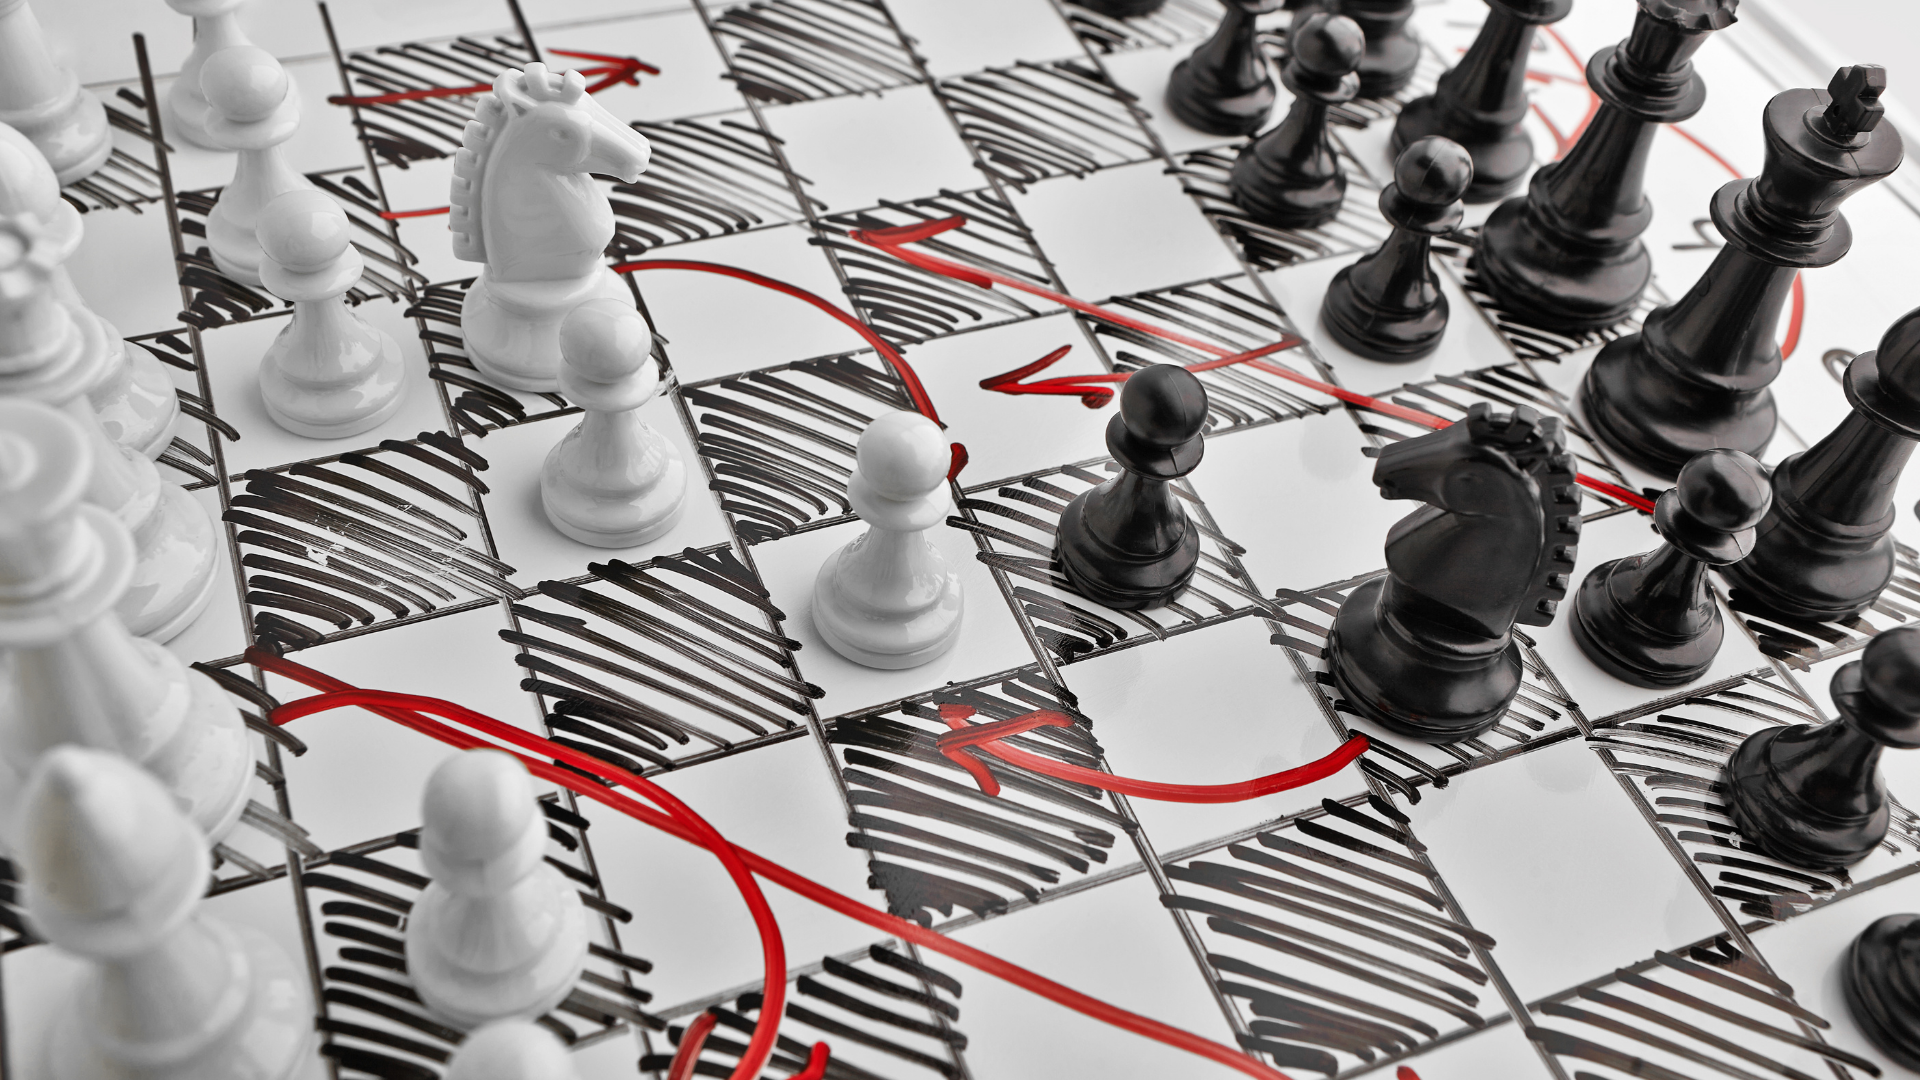
\includegraphics[width=\textwidth]{figures/motivation1.png}
            \caption{Playing chess}
        \end{figure}
    \end{column}
    \begin{column}{0.7\textwidth}  %%<--- here
        Goal: Win as much as possible!

        \begin{itemize}
            \item At time $t$, state $S_t$ is a position of all chess piecies.
            \item Agent at state $S_t$ can apply a valid move of one of its chess pieces.
            \item Environment dynamic: 
                \begin{itemize}
                    \item The opponent will move 1 of its piece.
                    \item Emits a reward of $0$ when the game is not terminated, otherwise $1$ for winning, $-1$ for losing,  $0$ for drawing.
                \end{itemize}
            \item Return $G_t = \sum^{\infty}_{k=1} R_{t+k+1}$.

        \end{itemize}
    \end{column}
    \end{columns}
\end{frame}

\begin{frame}
    \frametitle{RL Framework}
    \begin{figure}
        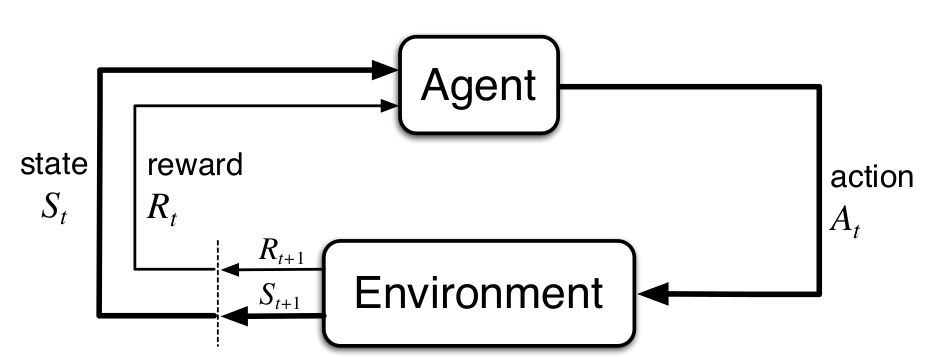
\includegraphics[width=0.4\textwidth]{figures/agent-environment.png}
        \caption{(ref. Book)}
   \end{figure}
   \textbf{Input of the framework}

   Environment - Agent interation:
   \begin{itemize}
       \item At time step $t$, \textit{agent} at state $S_t$ performs an action $A_t \in \mathcal{A}_t$
       \item {\color{blue} (2) Environment's dynamics.} The \textit{environment} acts accordingly change to state $S_{t+1}$, emits a reward $R_{t+1}$
       \item {\color{blue} (1) Episodic/Continuing task.} \textit{Return}: $G_t = \sum^{\infty}_{k=1} \gamma^{k}R_{t+k+1}$
   \end{itemize}
   \textbf{Output of the framework}

   {\color{blue} (3) How.} An agent that acts on the environment so that it maximizes the expectation of \textit{return}, i.e., $ \mathbb{E}[G_t]$.
\end{frame}

\begin{frame}
    \frametitle{(1) Episodic/Continuing tasks}
    The interation agent-environment produces $S_1, A_1, R_2, S_2, A_2, R_3, \ldots $
    \begin{columns}
        \begin{column}{0.5 \textwidth}
            \textbf{Episodic tasks}
            \begin{itemize}
                \item The sequence can break natually into subsequences
                \item Example: playing chess
                \item Return 
                    \[G_t = \sum^{{\color{red}T}}_{k=1} \gamma^{k} R_{t+k+1}, 0 \leq \gamma {\color{red}\leq} 1 \]
                \item There exits a termination state
            \end{itemize}
        \end{column}

        \begin{column}{0.5\textwidth}
            \textbf{Continuing tasks}
            \begin{itemize}
                \item Otherwise
                \item Example: Robot with long life span
                \item Return 
                    \[G_t = \sum^{{\color{red}\infty}}_{k=1} \gamma^{k} R_{t+k+1}, 0 \leq \gamma {\color{red}<} 1\]
                \item There is no notion of termination state
            \end{itemize}
        \end{column}
    \end{columns}
    % Key difference: the existence of termination state.

    $\quad \quad $ In both cases: $G_t = R_{t+1} + \gamma G_{t+1}$.
\end{frame}

\begin{frame}
    \frametitle{(2) Environment's dynamics}
    Markov decision process (MDP) descibes environment's dynamics
   \begin{itemize}
       \item Finite sets of states, action, rewards $\mathcal{S}, \mathcal{A}, \mathcal{R}$
       \item Random variables $S_t \in \mathcal{S}, R_t \in \mathcal{R}$ are only dependent on preceding state and action, i.e.,
           $ p(s', r | s, a) \coloneqq \text{Pr}(S_t = s', R_t = r | S_{t-1} = s, A_{t-1} = a)$ 
       \item \textbf{Markov property.} State must include all information of the past that makes a difference for the future
   \end{itemize}
\end{frame}

\begin{frame}
   Example: A recycling robot
   Describe more
   Some justication 

   Diff on agent and Env
    \begin{figure}
        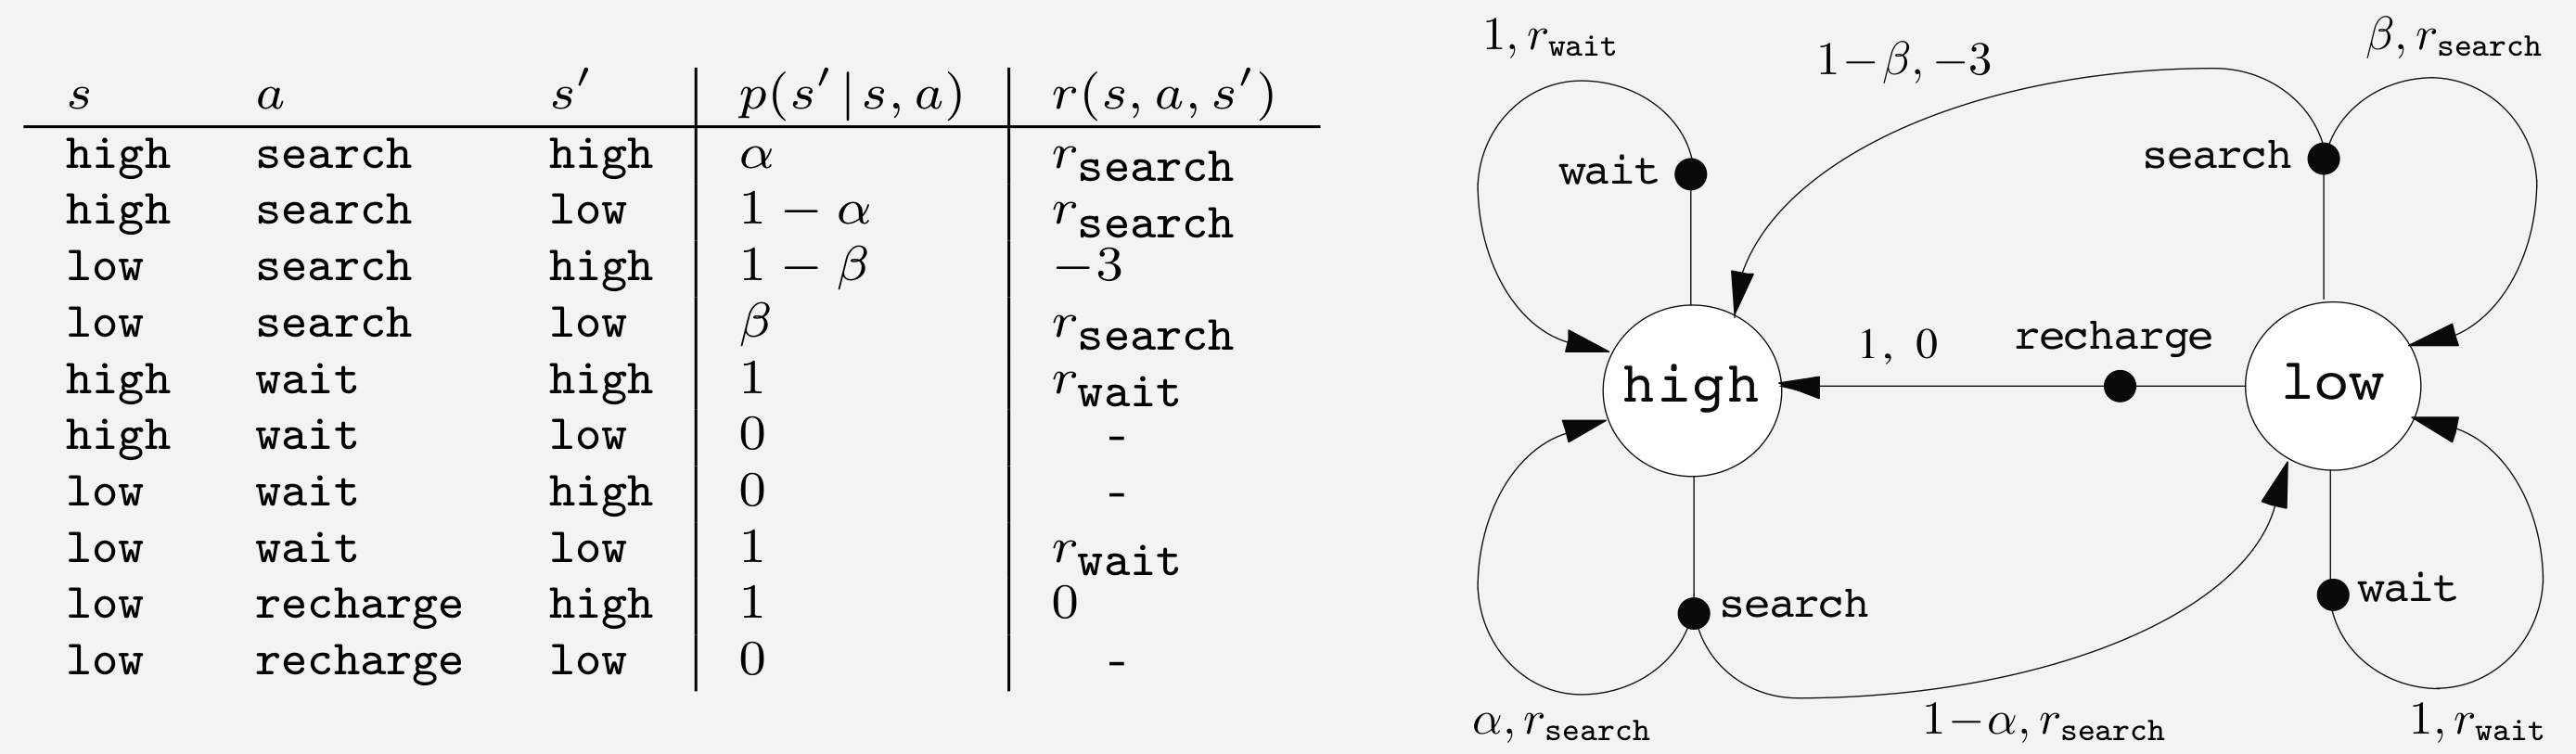
\includegraphics[width=0.8\textwidth]{figures/MDP_present.png}
        \caption{Example of an MPD}
    \end{figure}
\end{frame}


\begin{frame}
    \frametitle{(3) How. Part1: Evaluation --- Policy and Value function}
    \begin{itemize}
        \item Policy $\pi$ is a mapping from $\mathcal{S} \longrightarrow \mathcal{D}(a)$ where $\mathcal{D}(a)$ is some probability distribution over action space. If the agent follows policy $\pi$,  
            \[ \pi(a|s) = \text{Pr}(A_t =a| S_t = s)\]
        \item \textit{Value function} of a state under $\pi$, denoted $v_\pi(s)$, is the expected return when starting in $s$ and following $\pi$ thereafter, i.e.,
             \[
                 v_\pi(s) = \mathbb{E}_{\pi}[G_t | S_t =s] = \mathbb{E}_{\pi} \left[ R_{t+1} + \gamma G_{t+1} | S_t =s \right]
            \] 
        \item We call $v_\pi$  the \textit{state-value function for policy  $\pi$}
        \item Based on that, define the \textit{action-value function} for policy $\pi$ as
             \begin{align*}
                 q_\pi(s, a) &= \mathbb{E}_{\pi}[R_{t+1} + \gamma G_t | S_t =s, A_t = a] \\
                             &= \mathbb{E}_{\pi} \left[ R_{t+1} + \gamma G_{t+1} | S_t=s, A_t=a \right]
            \end{align*} 
    \end{itemize}
\end{frame}

\begin{frame}
    \frametitle{Bellman Equation of Value Function}
    \begin{align*}
         &v_\pi(s)  \\
         &= \mathbb{E}_{\pi}[G_t | S_t =s] = \mathbb{E}_{\pi} \left[ R_{t+1} + \gamma G_{t+1} | S_t =s \right] \\
         &= \sum_{a} \pi(a|s) \mathbb{E} \left[ R_{t+1} + \gamma G_{t+1} | S_t =s \right] \\
         &= \sum_{a} \pi(a|s) \sum_{s', r} p(s', r| S_t = s, A_t = a) \left[ r + \gamma G_{t+1} \right] \\
         &= \sum_{a} \pi(a|s) \sum_{s', r} p(s', r| S_t = s, A_t = a) \left( r + \gamma \mathbb{E}_\pi \left[ R_{t+2} + \gamma G_{t+2} | S_{t+1} = s' \right] \right) \\
        &= \sum_{a} \pi(a|s) \sum_{s', r} p(s', r| S_t = s, A_t = a) \left( r + \gamma v_\pi(s') \right)
    \end{align*}
    \begin{figure}
        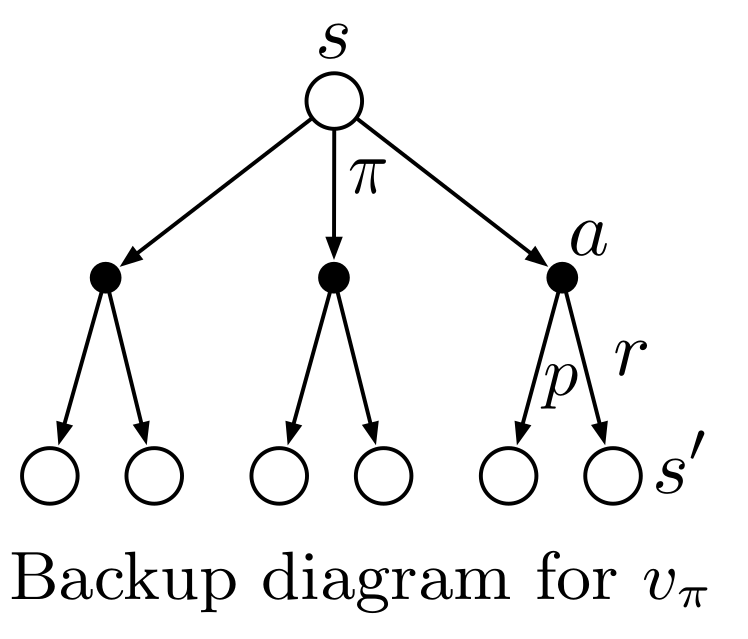
\includegraphics[width=0.2\textwidth]{figures/bellman_visual.png}
        \caption{Backup operation for state-value function}
    \end{figure}
\end{frame}

% \begin{frame}
%     \frametitle{Bellman Equation}
%     \begin{itemize}
%         \item Bellman equation for state value function
%             \[
%         v_\pi(s) = \sum_{a} \pi(a|s) \sum_{s', r} p(s', r| S_t = s, A_t = a) \left( r + \gamma v_\pi(s') \right)
%             \] 
%         % \item Bellman equation for action value function
%         %     \[
%         %         q_\pi(s, a) = \sum_{a} \pi(a|s) \sum_{s', r} p(s', r| S_t = s, A_t = a) \left( r + \gamma v_\pi(s') \right)
%         %     \] 
%     \end{itemize}
%
%     \begin{figure}
%         \centering
%         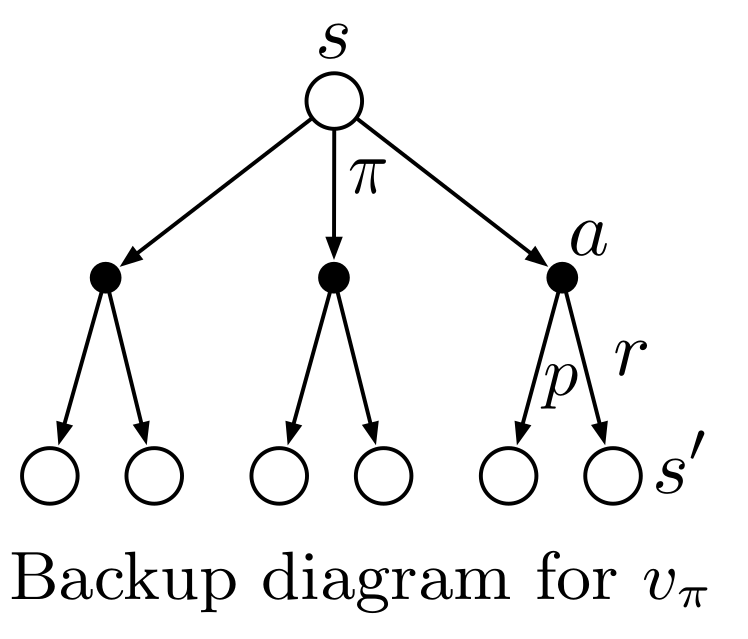
\includegraphics[width=0.3\textwidth]{figures/bellman_visual.png}
%         \caption{Backup operation for state-value function}
%     \end{figure}
% \end{frame}

\begin{frame}
    \frametitle{(3) How. Part 2: Optimal Policies}
    \begin{definition}
        A poicy $\pi$ is defined to be better than or equal to a policy $\pi'$ if its expected return is greater than or equal to that of  $\pi'$ for \textbf{all states}. In other words, 
        \[
        \pi \geq \pi' \Leftrightarrow v_\pi(s) \geq v_{\pi'} (s)  \text{ for all $s \in \mathcal{S}$} 
    \] 
    \end{definition}
    \begin{definition}
        $\pi_{\ast}$ is the \textit{optimal policy} if and only if $\pi_\ast \geq \pi$ for any  $\pi$. Value of optimal policy is called \textit{optimal state-value function}, denoted $v_\ast$ and defined as 
         \[
             v_\ast(s) \coloneqq \max_{\pi} v_\pi(s), \quad \text{for all } s \in \mathcal{S}
        \] 
        Similarly, $q_\ast(s, a)$ is \textit{optimal action-value function} and defined as
         \[
             q_\ast(s, a) \coloneqq \max_{\pi} q_\pi(s, a), \quad \text{for  all } s \in \mathcal{S}, a \in \mathcal{A}_t
        \] 
    \end{definition}
\end{frame}

\begin{frame}
    \frametitle{Bellman Optimality Equation}
    Assume $\pi_\ast$ exists,
    \begin{align*}
        v_{\ast} (s) 
        &= v_{\pi_\ast}(s) \quad \text{(by definition)}\\
        &= \max_{a \in \mathcal{A}(s)} \; q_{\pi_\ast}(a, s) \\
        &= \max_{a \in \mathcal{A}(s)} \; \mathbb{E}_{\pi_\ast} \left[ R_{t+1} + \gamma G_{t+1}| S_t = s, A_t = a \right] \\
        % &= \max_{a \in A} \sum_{a} \pi_{\ast}(a|s) \sum_{s', r} p(s', r| S_t = s, A_t = a)  \left[ r + \gamma G_{t+1} \right] \\
        % &= \max_{a \in A} \sum_{a} \pi_{\ast}(a|s) \sum_{s', r} p(s', r| S_t = s, A_t = a)  \left[ r + \gamma v_{\ast}(s') \right] \\
          &= \max_{a \in \mathcal{A}(s)} \; \mathbb{E} \left[ R_{t+1} + \gamma v_{\ast} (s')| S_t = s, A_t = a \right] \\
        \Rightarrow v_{\ast}(s) &= \max_{a \in \mathcal{A}(s)} \; \sum_{s', r} p(s', r|  S_t =s, A_t = a)  \left( r + \gamma v_{\ast} (s') \right) \numberthis \label{eq:bellman_optim}
    \end{align*}
    Compare to Bellman equation 
    \begin{equation*}
         v_\pi(s) = \sum_{a} \pi(a|s) \sum_{s', r} p(s', r| S_t = s, A_t = a) \left( r + \gamma v_\pi(s') \right) 
    \end{equation*}

    \textit{the equation (\ref{eq:bellman_optim}) doesn't depend on any particular policy}
\end{frame}



\begin{frame}
    \frametitle{Properties regarding Bellman Equations}
    \begin{gather}
        \label{eq:bellman_v1}
         v_\pi(s) = \sum_{a} \pi(a|s) \sum_{s', r} p(s', r| S_t = s, A_t = a) \left( r + \gamma v_\pi(s') \right)  \\
        \label{eq:bellman_v2}
        v_{\ast}(s) = \max_{a \in \mathcal{A}(s)} \; \sum_{s', r} p(s', r|  S_t =s, A_t = a)  \left( r + \gamma v_{\ast} (s') \right)
    \end{gather}
    \begin{remark}
        \label{remark:bellman}
        \begin{itemize}
            \item Bellman equation (\ref{eq:bellman_v1}) has an unique solution, which is $v_{\pi}(s)$.
            \item Bellman optimality equation (\ref{eq:bellman_v2}) has an unique solution, which is $v_\ast(s)$
        \end{itemize}
    \end{remark}
    Implication: 
    \begin{itemize}
        \item Given an optimal value function, \textit{greedy policy} is the optimal policy, (actions satisfies (\ref{eq:bellman_v2}))
        \item Given an optimal action-value function $q_{\ast}(s, a)$, the optimal policy is $ \argmax_{a} q_{\ast}(s, a)$
    \end{itemize}
\end{frame}

\begin{frame}
    Sketch proof of Remark \ref{remark:bellman}.
    Define 
    \begin{itemize}
    \item A fixed point of a function $f$ is  $x$ such that  $x = f(x)$
    \item An function $f: \mathbb{R}^{N} \rightarrow \mathbb{R}^{N}$ is called a contraction if there exists $0 < \alpha < 1$ such that
        \[
            \norm{f(\bm{s}) - f(\bm{s}')}_p \leq \alpha \norm{\bm{s} - \bm{s}'}_p, \quad \text{ for some $p \geq 1$}
        \] 
    \end{itemize}
    \begin{enumerate}
    \item If $f$ is an $\alpha$-contraction, then $f$ has an unique fixed point
    \item Let $\bm{v} \in \mathbb{R}^{N}$ be a vector of all value states, 
        \begin{align*}
            T_{\pi}(\bm{v})[s] &\coloneqq \sum_{a} \pi(a|s) \sum_{s', r} p(s', r| S_t = s, A_t = a) \left( r + \gamma v_\pi(s') \right)  \\
        T_{\ast}(\bm{v})[s] &\coloneqq \max_{a \in \mathcal{A}(s)} \; \sum_{s', r} p(s', r|  S_t =s, A_t = a)  \left( r + \gamma v_{\ast} (s') \right)
        \end{align*} 
        $T_{\pi}, T_{\ast}$ are both contraction.
    \end{enumerate}
\end{frame}

\begin{frame}
    \frametitle{Step 1}
    If $f$ is a $\alpha$-contraction, then  $f$ has an unique fixed  point.

     \begin{proof}
        \textbf{Uniqueness}
        Let $\bm{s}, \bm{s}'$ are 2 fixed points of $f$.
         \[
             \alpha \norm{\bm{s} - \bm{s}'}_p \geq \norm{f(\bm{s}) - f(\bm{s}')}_p = \norm{\bm{s} - \bm{s}'}_p
        \] 
        Since $0 < \alpha <1 $, this contraction leads to $\bm{s} = \bm{s}'$.

        \textbf{Existence}
        \begin{itemize}
            \item Define a sequence of $\bm{s}_k$ such that $\bm{s}_{k+1} = f(\bm{s}_k)$
                \begin{align*}
                    \norm{\bm{s}_{k+1} - \bm{s}_k}_p
                    &= \norm{f(\bm{s}_k) - f(\bm{s}_{k-1})}_p  \\
                    &\leq \alpha \norm{\bm{s}_k - \bm{s}_{k-1}}_p
                    = \alpha \norm{f(\bm{s}_{k-1}) - f(\bm{s}_{k-2})}_p  \\
                    &\leq \alpha^2 \norm{\bm{s}_{k-1} - \bm{s}_{k-2}}_p \leq \ldots \leq \alpha^{k} \norm{\bm{s}_1 - \bm{s}_0}_p
                \end{align*} 
            \item Intuitively, we can say that $\bm{s}_{\ast} = \lim_{k \rightarrow \infty} \bm{s}_{k}$ for some $\bm{s}_{\ast}$, hence $\bm{s}_{\ast} = f(\bm{s}_{\ast})$. Technically, it involes of showing domain of $f$ is complete and sequence ${\bm{s}_k}$ is a Cauchy sequence.
        \end{itemize}
    \end{proof}
\end{frame}

\begin{frame}
    \frametitle{Step 2}
    $T_{\pi}$ is a $\gamma$-contraction with $p = \infty$.

     \begin{proof}
         \begin{align*}
             \abs{T_{\pi}(\bm{v})[s] - T_{\pi}(\bm{v}')[s]} 
             &= \abs{ \sum_{a \in \mathcal{A}(s)} \sum_{s', r} \gamma \pi(a|s) p(s', r| s, a) (\bm{v}[ s' ] - \bm{v}'[ s' ]) }    \\
             & \leq  \abs{ \sum_{a \in \mathcal{A}(s)} \sum_{s', r} \gamma \pi(a|s) p(s', r| s, a) \max_{s} (\bm{v}[ s ] - \bm{v}'[ s ]) }    \\
             & \leq  \abs{   \gamma \max_{s } (\bm{v}[ s ] - \bm{v}'[ s ]) }    \\
             & =    \gamma \norm{ \bm{v} - \bm{v}' }_{\infty}    \\
         \end{align*} 
    \end{proof}
    Similar proof for $T_{\ast}$. 

    Since $T_{\pi}, T_{\ast}$ are  contraction and there exists unique points $v_{\pi}, v_{\ast}$, they are unique.
\end{frame}

\begin{frame}
    \frametitle{(3) How. Part 3: Find optial policy}
    Next session.
\end{frame}

\begin{frame}
    \frametitle{Reference}
    \begin{itemize}
        \item Sutton, Richard S., and Andrew G. Barto. Reinforcement learning: An introduction. MIT press, 2018.
        \item The notes\footnotemark by Dr Daniel Murfet
    \end{itemize}
    \footnotetext[1]{http://therisingsea.org/notes/mast30026/lecture14.pdf}
\end{frame}

\end{document}

